\documentclass[
  a4paper,            % DIN A4
  DIV=10,             % Schriftgröße und Satzspiegel
  oneside,            % einseitiger Druck
  BCOR=5mm,           % Bindungskorrektur
  parskip=half,       % Halber Abstand zwischen Absätzen
  numbers=noenddot,   % Kein Punkt hinter Kapitelnummern
  bibtotoc,           % Literaturverzeichnis im Inhaltsverzeichnis
  listof=totoc        % Abbildungs- und Tabellenverzeichnis im Inhaltsverzeichnis
]{scrreprt}
\usepackage{../style/thesisstyle}

%\usepackage{layout}       % Layout Debugging
%\usepackage{showframe}    % Layout Debugging
\usepackage{lipsum}       % for example only
\usepackage{blindtext}    % for example only

\usepackage{float}
\usepackage{pifont}
\usepackage{listings}
\usepackage{color}
\usepackage{caption}
\usepackage{bbding}

\newcounter{nalg}[chapter] % defines algorithm counter for chapter-level
\renewcommand{\thenalg}{\thechapter \arabic{nalg}} %defines appearance of the algorithm counter
\DeclareCaptionLabelFormat{algocaption}{Algorithmus \thenalg} % defines a new caption label as Algorithm x.y

\lstnewenvironment{algorithm}[1][] %defines the algorithm listing environment
{
  \refstepcounter{nalg} %increments algorithm number
  \captionsetup{labelformat=algocaption,labelsep=colon} %defines the caption setup for: it ises label format as the declared caption label above and makes label and caption text to be separated by a ':'
  \lstset{ %this is the stype
    mathescape=true,
    frame=tB,
    numbers=left,
    numberstyle=\tiny,
    basicstyle=\scriptsize,
    keywordstyle=\color{black}\bfseries\em,
    keywords={,input, output, return, datatype, function, in, if, else, foreach, while, begin, end, } %add the keywords you want, or load a language as Rubens explains in his comment above.
    numbers=left,
    xleftmargin=.04\textwidth,
    #1 % this is to add specific settings to an usage of this environment (for instnce, the caption and referable label)
  }
  \lstset{literate=%
      {Ö}{{\"O}}1
      {Ä}{{\"A}}1
      {Ü}{{\"U}}1
      {ß}{{\ss}}1
      {ü}{{\"u}}1
      {ä}{{\"a}}1
      {ö}{{\"o}}1
  }
}
{}

\makeglossaries           % create all glossary entries (remember: run makeglossaries manually)
\loadglsentries{thesisglossaries.tex}  % load acronym, symbol and glossarie entries

\begin{document}
% !TEX root = ../thesis.tex
%
% configurations
%

% text field
%-> replace supervisor names with correct ones
\firstSupervisor{Prof. Dr. Philipp Jenke}
\secondSupervisor{Prof. Dr. Michael Neitzke}

% text field
%-> replace title with your thesis title
\thesisTitle{Template-basierte Synthese von Verzweigungsstrukturen mittels L-Systemen}
\thesisTitleEN{Template-based synthesis of branching structures using L-Systems}

% text field
%-> replace the key words with your own key words
\keywordsDE{Verzweigungsstruktur, 2D Generierung, L-System, Template, Prozedurale Modellierung, Inverse Prozedurale Modellierung, Baumstruktur, Formale Grammatik, Ähnlichkeit}
\keywordsEN{Branching Structure, 2D Generation, L-System, Template, Procedural Modeling, Inverse Procedural Modeling, Tree Structure, Formal Grammar, Similarity}

% text field
%-> replace the text with a description of the thesis
\abstractDE{
Prozedurale Modellierung beschreibt effiziente Methoden zur Erzeugung einer Vielzahl
an Modellen nach bestimmten Regeln. Die Erstellung eines Systems zur Umsetzung solcher Methoden ist durch
einen Mangel an Kontrolle und einer geringen Vorhersagbarkeit der Ergebnisse erschwert.
Diese Bachelorarbeit präsentiert ein System zur Synthese von Verzweigungsstrukturen, die einer benutzerdefinierten
Strukur ähnlich sind. Dabei wird gezeigt, wie sich aktuelle Ansätze der Forschung in einem Programm umsetzen lassen.
Templates werden eingelesen und vom Benutzer zu einer Basisstruktur organisiert.
Anschließend wird ein L-System über die Topologie dieser Struktur inferiert, komprimiert und dann generalisiert.
Nach der Interpretation des L-Systems können vom Benutzer gesetzte Transformationsparameter aus einer Häufigkeitsverteilung
angewendet werden. Zum Schluss wird die resultierende Verzweigungsstruktur visualisiert.
}
\abstractEN{
Procedural modeling describes efficient methods for creating various models after certain rules.
Setting up a system, that implements such methods, lacks of controllability and predictability of the results
and is therefore a difficult task. This bachelor thesis presents a system for synthesizing branching structures
that are similar to custom structures created by a user. It is shown how current research can be implemented into a
program. Templates are used to be organized into a basic structure. Then the topology gets inferred, compressed and
generalized into an L-System. After deriving the L-System, custom transformation parameters from a frequency distribution
can be applied. Finally, the resulting branching structure is visualized.
}

% text field
%-> replace jon with your name
\thesisAuthor{Adrian Helberg}

% text field
%-> enter the submission date
\submissionDate{\today}

% switch - uncomment only one
%-> uncomment NDA or public
%\NDA{yes}
\NDA{no}

%-> uncomment cover or cover Corporate Design 2017
\Cover{CD2017}
%\Cover{CD2017NoLogo}
%\Cover{Std2018}

% switch - uncomment only one
%-> uncomment to show list of figures or not
\ListOfFigures{yes}
%\ListOfFigures{no}

% switch - uncomment only one
%-> uncomment to show list of tables or not
\ListOfTables{yes}
%\ListOfTables{no}

% switch - uncomment only one
%-> uncomment to show list of accronyms or not
\ListOfAccronyms{yes}
%\ListOfAccronyms{no}

% switch - uncomment only one
%-> uncomment to show list of symbols or not
\ListOfSymbols{yes}
%\ListOfSymbols{no}

% switch - uncomment only one
%-> uncomment to show list of glossary entries or not
\Glossary{yes}
%\Glossary{no}

% switch - uncomment only one
%-> uncomment the study course you are in
%\studycourse{ITS}
%\studycourse{TI}
\studycourse{AI}
%\studycourse{WI}
%\studycourse{EI}
%\studycourse{REE}
%\studycourse{BMT}
%\studycourse{MAI}
%\studycourse{MIK}
%\studycourse{MA}
    % load all settings

%\layout{}                 % Layout Debugging

\hyphenation{Ba-che-lor-the-sis Mas-ter-the-sis}

% Cover page here, no page number
\ICoverPage

% PDF Metadata
% !TEX root = ../thesis.tex
%
% PDF Metadata integration
% @author Thomas Lehmann
%

% PDF Metadata
\hypersetup{
pdftitle={\IthesisTitle},
pdfauthor={\IthesisAuthor},
pdfkeywords={\IkeyWordsEN}
}

% Titlepage is page one even if the number is not shown.
\pagenumbering{roman}
% Title page here
% !TEX root = ../thesis.tex
%
% title page
% @author Thomas Lehmann
% Hints for title page and page numbering: https://en.wikipedia.org/wiki/Title_page
%
\title{\IthesisTitle}   % set latex default title to be used by hyperref in pdf
\author{\IthesisAuthor} % set latex default author to be used by hyperref in pdf

\newpage
\thispagestyle{empty}
{\fontfamily{phv}\selectfont
  \hfuzz=20pt       % suppress warnings due to extenstion onto page margins

  % Author of thesis
  \vspace*{1cm}
  \begin{minipage}[b]{\textwidth}
    \fontsize{14pt}{20pt}
    \selectfont
    \begin{center}
      \IthesisAuthor
    \end{center}
  \end{minipage}

  % Title of thesis
  \vspace{1.5cm}
  \begin{minipage}[b][0cm][t]{\textwidth}
    \fontsize{18pt}{20pt}
    \selectfont
    \begin{center}
      \IthesisTitle
    \end{center}
  \end{minipage}

  % Important information
  \begin{textblock*}{\textwidth}(40mm,210mm)
    \begin{minipage}[b]{\textwidth}
      \hbadness=10001    % suppress underfull warning due to short text
      \fontfamily{cmr}\selectfont
      \fontsize{12pt}{14pt}
      \selectfont
      \IthesisKindDE ~eingereicht im Rahmen der \IthesisExaminationDE \\
      im Studiengang \textit{\IstudyCourseName} \\
      am \IthesisDepartmentFull \\
      der Fakultät Technik und Informatik\\
      der Hochschule für Angewandte Wissenschaften Hamburg\\

      Betreuender Prüfer: \IfirstSv \\
      Zweitgutachter: \IsecondSv \\

      Eingereicht am: \ISubDate \\
    \end{minipage}
  \end{textblock*}
}


% Abstract page here
% !TEX root = ../thesis.tex
%
% abstract page
% @author Thomas Lehmann
%
\newpage
\thispagestyle{plain}
\clearpage
\hfuzz=12pt       % suppress warnings due to extenstion onto page margins

\textbf{\IthesisAuthor}

\vspace{0.3cm}
\textbf{Thema der Arbeit}

\IthesisTitle

\vspace{0.3cm}
\textbf{Stichworte}

\IkeyWordsDE

\vspace{0.3cm}
\textbf{Kurzzusammenfassung}

\begin{minipage}{\textwidth}
\IabstractDE
\end{minipage}

\vspace{1.0cm}
\textbf{\IthesisAuthor}

\vspace{0.3cm}
\textbf{Title of Thesis}

\IthesisTitleEN

\vspace{0.3cm}
\textbf{Keywords}

\begin{minipage}{\textwidth}
\IkeyWordsEN
\end{minipage}

\vspace{0.3cm}
\textbf{Abstract}

\IabstractEN


% Table of contents here
\tableofcontents

% List of figures here
\IListOfFigures

% List of tables here
\IListOfTables

% List of accronyms here
\IListOfAccronyms

% List of symbols here
\IListOfSymbols

% Uncomment if list of source code is needed (rarely).
\lstlistoflistings  % requires package listings, needs to uncommenting of usepackage

% path to the chapters folder is set to find the images used there
\graphicspath{ {./chapters/} }

% Chapters
\clearpage
\pagenumbering{arabic}
% @author Arian Helberg

\chapter{Einleitung}

\gls{ac:haw}~\gls{sy:ohm}~\gls{gl:haw}(Damit das glossar keine fehler schmeißt)

Effizientes Objektdesign und -modellierung sind entscheidende Kernkompetenzen in verschiedenen Bereichen der
digitalen Welt.
Da die Erstellung geometrischer Objekte für Laien unintuitiv ist und ein großes Maß an Erfahrung und Expertise
erfordert, ist dieses stetig wachsende Feld für Neueinsteiger nur sehr schwer zu erschließen.
Die Forschung liefert hierzu einige Arbeiten zur prozeduralen Modellierung, um digitale Inhalte schneller
und automatisiert zu erstellen.
Gerade wenn es um die Darstellung natürlicher Umgebung geht, ist die Erstellung von ähnlichen Objekten, wie
zum Beispiel verschiedene Bäume derselben Gattung eines Waldes, ein schwieriges Problem.
Kleine Änderungen in prozeduralen Systemen können zu großen Veränderungen der Ergebnisse führen.
Darum beschäftigt sich die inverse prozedurale Modellierung unter anderem mit dem Inferieren von Regeln
und Mustern aus gegeben Objekten, um diese nach bestimmten Regeln zu modellieren.
Ein wichtiges Werkzeug hierbei ist die Verwendung formaler Grammatiken als fundamentale Datenstruktur
der Informatik, um Strukturen zu beschreiben.
Eine spezielle Untergruppe sind die L-Systeme, die häufig bei der Beschreibung
von Verzweigungsstrukturen und Selbstähnlichkeit zum Einsatz kommen.
\\~\\
Diese Arbeit soll sich mit der Erstellung eines prozeduralen Systems zur Synthese von Ähnlichkeitsabbildern
beschäftigen.
Hierzu soll über eine Benutzerschnittstelle eine Struktur erzeugt werden, aus der ein parametrisiertes L-Systems
inferiert werden kann, das dann zur Generierung von ähnlichen Strukturen genutzt werden kann.

\newpage

\section{Problemstellung}

Mit der Digitalisierung der Welt steigt auch der Bedarf an digitalen Inhalten.
Zu den größten Feldern gehören Gaming- und Unterhaltungsindustrie, Datenvisualisierung und interaktive Anwendungen.
Um eine erhöhte Quantität dieser Inhalte liefern zu können, werden Methodiken und Algorithmen gesucht, die eine Erstellung
vereinfachen.
Während Methodiken zur Kodifizierung bestimmter Strukturen in den Bereich der prozeduralen Modellierung fällt,
findet das Ableiten von Regeln Anwendung in der inversen prozeduralen Modellierung.
Weiter steigt mit dem digitalen und naturwissenschaftlichen Fortschritt die Anwendung immer komplexerer Strukturen, die
ein Herausarbeiten der schwer zu kontrollierenden, prozeduralen Regeln immer schwieriger machen.
\\~\\
Ein Beispiel hierzu aus der Gaming-Industrie ist die frühere Verwendung unorganisierter Modelle.
Unorganisierte Modelle sind nur bedingt wiederverwendbar, da nur die vorliegende Modellierung verwendet werden kann.
Es besteht eine hohe Speicherkomplexität bei geringer Laufzeitkomplexität.
Für kleinste Veränderungen am Modell ist eine erneute Modellierung nötig, die wiederum Speicher benötigt, um sie
persistent speichern zu können.
Heutzutage werden die Objekte nach bestimmten Kriterien organisiert, um eine austomatisierte Modellierung durch Algorithmen
zu ermöglichen, um so aus einer Grundstruktur weitere Modelle zu erzeugen.
Speicher- und Laufzeitkomplexität nähern sich an.
Deshalb werden allgemeingültige, vielseitig anwendbare Algorithmen gesucht, die bestimmte natürliche Eigenschaften
von Strukturen herausarbeiten ("`Reverse Engineering"'), um diese für die (inverse) prozedurale Modellierung zur
Verfügung zu stellen.
\\~\\
Diese Arbeit soll zeigen, wie sich durch die Erstellen eines Systems zur Generierung von ähnlichen Strukture aus einer
Basistruktur aktuelle Ansätze aus der Forschung in einem Programm umsetzen lassen.

\newpage

\section{Ziele}

Die Erstellung eines Systems zur Synthese von ähnlichen Struktures aus einer Basisstruktur soll zentrale Aufgabe dieser
Arbeit sein.
Aus der Fragestellung leiten sich folgende Teilziele ab:

\begin{itemize}
    \item Die Erstellung eines Programms zur Umsetzung des erstellten Systems
    \item Anwenden von Algorithmen und Ansätzen der aktuellen Forschung
    \item Testen von Metriken und deren Auswirkung auf das Ergebnis
    \item Erstellung eigener Methodiken und Algorithmen zur Effizienten Lösung der Problemstellung
    \item Schaffen eines Teilsystems zum Extrahieren von Eigenschaften und Regeln einer Basisstruktur
\end{itemize}

Die Erstellung und Integration eines neuronalen Netzes, das laut aktueller Forschung gute Ergebnisse beim Lernen von
Regeln aus einer Eingabestruktur liefert, kann in dieser Arbeiten aus Praktikabilitätsgründen nicht behandelt werden.

\section{Methodik}
Der Benutzer des Systems legt atomare Strukturen in Form von Zeichenketten an, die vom Programm eingelesen und
als Templates zur Verfügung gestellt werden.
Die Templates sind beliebig und können eine einfach Linie oder eine komplexe Verzweiung darstellen.
Werden diese Strukturen auf der graphischen Oberfläche platziert und mit diversen Transformationen verändert, spricht man
von Instanzen oder Template-Instanzen.

\subsection*{Strukturieren}
Der Benutzer nutzt die grafische Benutzerschnittstelle, um aus einzelnen Templates eine zusammenhängende Basisstruktur zu
erstellen.
Neben der Position der Instanzen werden Transformationensparameter, wie Rotation oder Skalierung, angepasst.

\subsection*{Visualisieren}
Der aktuelle Stand der Strukturierung ist jederzeit sichtbar.
Liniensegmente und Bindungselemente werden in einem graphischen Element visualisiert und für eine Interaktion zur Verfügung
gestellt.

\subsection*{Datenaufbereitung}
Das Ergebnis der Strukturierung wird in einer Baumstruktur
organisiert, in der jeder Knoten einer bestimmten Template-Instanz entspricht und die eingehenden Kanten die
geometrischen Transformationen relativ zum Elternknoten beschreibt.

\subsection*{Inferieren}
Aus der Baumstruktur kann eine formale Grammatik in Form eines L-Systems abgeleitet werden.
Diese Grammatik beschreibt lediglich die erstellte Basisstruktur und beinhaltet keine Transformationsparameter, da hier
nur auf die Topologie des Baumes und nicht auf geometrische Unterschiede der Instanzen eingegangen wird.

\subsection*{Komprimieren}
Um sich wiederholende Produktionregeln zu vermeiden und so sowohl das Alphabet, als auch die Produktionsregelmenge
zu kompromieren, wird die Baumstrukturen nach identischen, maximalen Unterbäumen durchsucht und durch zusammengefasste
Instanzen vereinfacht.
Hierbei gilt die Baumstruktur selbst nicht als Unterbaum.

\subsection*{Generalisieren}
Ähnliche Produktionsregeln des L-Systems werden mithilfe einer Kostenfunktion zusammengefasst, um dises mit
nicht-deterministischen Regeln und Rekursion zu generalisieren.

\subsection*{Randomisieren}
Jedes Symbol der Grammatik nimmt eine Liste an Parametern entgegen, die nach bestimmten Kriterien pseudo-randomisiert
werden, um Variationen von Template-Instanzen zu erstellen.
Das Ausführen des L-Systems kann nun Ähnlichkeitsstrukturen für die Basisstruktur erzeugen.

\section{Aufbau}

Die Methodik zum Umsetzen des beschriebenen Systems wird wie folgt umgesetzt.

\begin{figure}[H]
    \centering
    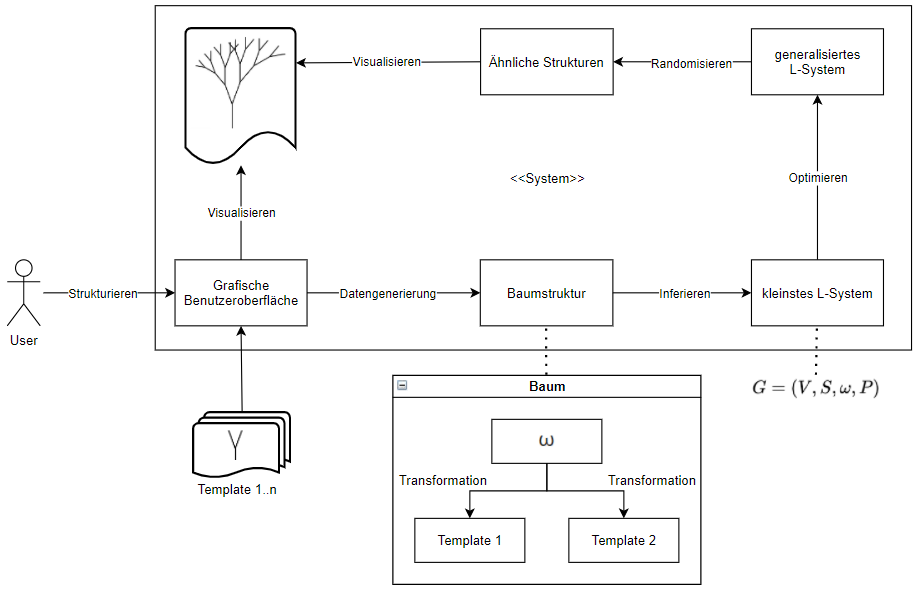
\includegraphics[width=14cm]{../images/System.PNG}
    \caption[Systemarchitektur]{Architektur des Systems mit einigen Datenstrukturen}
\end{figure}

Die Darstellung zeigt eine grobe Übersicht der Anwendungsfälle innerhalb des Systems.
Der Benutzer strukturiert vom System importierte Templates zu einer Basisstruktur mittels grafischer Bedienelemente.
Die Template-Instanzen werden hierbei in einer Baumtopologie organisiert.
Anschließend wird ein L-System aus der Baumstruktur generiert und komprimiert.
Bevor randomisierte, geometrische Parameter auf das kompakte L-System angewendet werden, wird dieses generalisiert.
Zuletzt wird das Axiom des abgeleiteten L-Systems durch die Ausführung erweitert und sichtbar gemacht.
% @author Arian Helberg

\chapter{Grundlagen}

Die Modellierung mithilfe von Grafiksoftware ist eine vergleichbar händische, langwierige Erstellung von
Objekten.
Hierbei hat der Designer (Modellierer) die volle Kontrolle über die Strukturen des Objektes.\\
Bei der prozeduralen Modellierung werden spezifische Strukturen eines zu erstellenden physikalischen Objektes
generalisiert und meist über eine Grammatik und globale Parameter abgebildet.
Während bei der klassischen Modellierung die menschliche Intuition und bei der prozeduralen Modellierung eine
parametrisierte Grammatik genutzt werden kann, arbeitet die inverse prozedurale Modellierung mit bestehenden Modellen und
extrahiert ("`lernt"') die Strukturen des Objektes, die automatisch in eine formale Grammatik überführt werden können.
Die Generierung von prozeduralen Modellen ist ein wichtiges, offenes Problem~\cite{benes_2011}.

\section{Grundbegriffe}

\subsection*{Modellierung}
Um einen physikalischen Körper in ein digitales Objekt zu überführen, wird mithilfe von Abstraktion (Modellierung)
ein mathematisches Modell erstellt, das diesen Körper formal beschreibt.
3D Grafiksoftware, wie bspw. Blender~\cite{blender}, wird genutzt um geometrische Körper zu modellieren, texturieren
und zu animieren.

\newpage

\subsection*{Prozedurale Modellierung}
\begin{quote}
    "`It encompasses a wide variety of generative techniques that
    can (semi-−)automatically produce a specific type of content based on a set of input
    parameters"'~\cite{smelik_2014}
\end{quote}
Prozedurale Modellierung beschreibt generative Techniken, die \\(semi-)automatisch spezifische, digitale
Inhalte anhand von deskriptiven Parametern erzeugen.
\citeauthor{smelik_2014} beschreibt einen Prozess, welcher durch das Nutzen globaler Parameter und descriptiven Regeln
Modelle erzeugt~\cite{smelik_2014}.
\subsection*{Inverse prozedurale Modellierung}
\citeauthor{aliaga_2016} spricht bei der inversen prozeduralen Modellierung von dem Finden einer prozeduralen Repräsentation
von Strukturen bestehender Modelle~\cite{aliaga_2016}.
Die Methodik aus Strukturen bestimmte Regeln und Parameter abzuleiten ist der Hauptgegenstand dieses Feldes der
Computergrafik und aktueller Gegenstand der Forschung.

\section{Grundlegende Arbeiten}

\citeauthor{smelik_2014} untersucht prozedurale Methoden, um diverse Strukturen, wie Vegetation, Straßen u.v.m zu erzeugen.
Es wird ein Überblick aktueller, vielversprechender Studien gegeben, deren Anwendung sowohl in technischen Bereichen,
als auch in nicht-technischen, kreativen Bereichen, diskutiert wird.
Diese Übersicht gilt als grundlegender Einstiegspunkt in die Bereiche der prozeduralen
Modellierung~\cite{smelik_2014}.
Einen aktuellen Stand der Forschung der inversen prozeduralen Modellierung (IPM) liefert~\citeauthor{aliaga_2016}.
Es wird gezeigt, dass IPM-Ansätze in entsprechende Kernprobleme der Informatik aufgeteilt und meist getrennt voneinander durch
verschiedene Methodiken und Algorithmen bearbeitet werden~\cite{aliaga_2016}.
Weiter wird ein Einblick in die Kategorisierung und Bewertung einiger Ergebnisse von IPM-Systemem gegeben.
\citeauthor{higuera_2010} weist darauf hin, dass ein wesentlicher Unterschied zwischen der Induktion einer Grammatik
und der Grammatikinferierung besteht~\cite{higuera_2010}.
Die Induktion beschreibt das Finden einer Grammatik, welche ein Datum am genauesten beschreibt.
Die Gammatikinferierung ist das Finden einer Grammatik, die eine bestimmte Zeichenfolge abdeckt.

\newpage

\citeauthor{higuera_2010} ordnet die inverse Generierung von L-Systemen zum Problem der Grammatikinferenz, welches er
als gut erforschtes Gebiet beschreibt.
Verzweigungsstrukturen im Kontext der inversen prozeduralen Modellierung tauchen in wissenschaftlichen Studien wenig auf.
~\citeauthor{guo_2020} adressiert einige IPM-Ansätze in seiner Arbeit~\cite{guo_2020}:\\~\\
Die Anwendung von modellierten Bäumen und Landschaften in den Bereichen wie Simulation, VR, Botanik und Architektur
wird in der Arbeit von \citeauthor{deussen_2010} gezeigt~\cite{deussen_2010}.
Hier geht es hauptsächlich um die Erstellung und Kombination künstlicher Modelle, um natürlich wirkende Umgebungen zu
schaffen.\\~\\
Mit der Erkennung von Wiederholungsmustern in Hausfassaden beschäftigt sich~\citeauthor{alhalawani_2013}.
Durch das Finden diverser Verformungsparameter mithilfe einer faktorisierten Fassadendarstellung werden neue
Bildbearbeitungsmöglichkeiten  vorgestellt~\cite{alhalawani_2013}.\\~\\
Ein virtueller Wiederaufbau der archäologischen Stätte von Pompeji mithilfe der Erstellung von Gebäudemodellen wird
von~\citeauthor{mueller_2006} vorgestellt.\\~\\
Das Modellieren ganzer Städte über das \texttt{CityEngine}-System wird in der Arbeit von ~\citeauthor{parish_2001}
gezeigt.
Zunächst werden geografische Bilder eingelesen, aus welchen dann die Anordnung von Straßen, Gärten und Gebäude
ausgelesen werden können.
Anschließend können virtuelle Städte nach dem Vorbild der Eingabe erstellt werden.\\~\\
Sowohl ~\citeauthor{merrell_2011}, als auch ~\citeauthor{zhang_2019} stellen Systeme zur Erzeugung von Inneneinrichtung
vor.
Über ein Layout-System werden Design Patterns gelernt, in Terme eine Dichtefunktion überführt, um dann virtuelle
Möbel zu erstellen~\cite{merrell_2011}.
Eine Übersicht über diverse Kriterien, die zur Erstellung von Innenraumszenen nötig sind, zeigt die
Wichtigkeit über die Auswahl sinnvoller Objekte und deren Anordnung um plausible Räume zu erstellen~\cite{zhang_2019}.

\newpage

\subsection*{L-Systeme}
\citeauthor{lindemayer_1968} führt eine mathematische Beschreibung zum Wachstum fadenförmiger Organismen ein.
Sie zeigt, wie sich der Status von Zellen infolge ein oder mehrerer Einflüsse verhält~\cite{lindemayer_1968}.
Weiter führt er Ersetzungssysteme ein, die atomare Teile mithilfe von Produktionsregeln ersetzen.
Diese L-Systeme nutzt er zur formalen Beschreibung von Zellteilung.
Später werden Symbole zur formalen Beschreibung von Verzweigungen, die von Filamenten abgehen, eingeführt~\cite{prusinkiewicz_1990}.
Die bekanntesten L-Systeme sind zeichenketten-basiert und werden von \textit{Noam Chomsky} eingeführt~\cite{chomsky_1956}.
Sie ersetzen parallel Symbole eines Wortes, die von einer Grammatik über eine Sprache akzeptiert werden.
L-Systeme können unter anderem parametrisiert oder nicht-parametrisiert und kontextfrei oder kontextsensitiv sein.

L-Systeme sind Grammatiken mit folgender Form:
\begin{center}
    $\mathcal{L}=\langle M,\omega,R \rangle$, mit
    \begin{itemize}
        \item $M$ als Alphabet, das alle Symbole enthält, die in der Grammatik vorkommen,
        \item $\omega$ als Axiom oder "`Startwort"' und
        \item $R$ als Menge aller Produktionsregeln, die für $\mathcal{L}$ gelten
    \end{itemize}
\end{center}
Das Alphabet eines parametrisierten Systems enthält Module (Symbole mit Parametern) anstatt Symbole:
\begin{center}
    $M=\{A(P),B(P),\dots\}$ mit
    \begin{itemize}
        \item $P=p_1,p_2,\dots$ als Modulparameter
    \end{itemize}
\end{center}
Zeichen des Alphabets, die Ziel einer Produktionsregel sind, heißen Variablen oder Nonterminale.
Alle anderen Zeichen aus $M$ sind Konstanten oder Terminale.
Das Axiom $\omega$ ist eine nicht-leere Sequenz an Modulen aus $M^+$ mit
\begin{itemize}
    \item $M^+$ als Menge aller möglichen Zeichenketten aus Modulen aus $M$
\end{itemize}
Produktionsregeln sind geordnete Paare aus Wörtern über dem Alphabet, die bestimmte Ersetzungsregeln umsetzen.
Hierbei werden Symbole aus einem Wort, die einer linke Seite (\textit{engl. left hand side (LHS)}) einer
Produktionsregel entsprechen, durch die rechten Seite (\textit{engl. right hand side (RHS)}) ersetzt.
Sie sind folgendermaßen aufgabaut:
\begin{center}
    $A(P)\rightarrow x,x\in M^*$, mit
    \begin{itemize}
        \item $M^*$ als die Menge aller möglichen Zeichenketten von M inklusive der leeren Zeichenkette $\varepsilon$
    \end{itemize}
\end{center}
Ist die RHS jeder Produktionsregel ein einzelnes Symbol und gibt es zu jeder Variablen eine Regel, spricht man
von einem kontextfreien, andernfalls von einem kontextsensitiven L-System.

\subsubsection*{L-System Interpretation}
Lindenmayer-Systeme können Worte über ihr Alphabet interpretieren.
Dafür werden Symbole des Wortes, die Ziel einer Produktionsregeln sind, in Iterationen durch die RHS
der Produktionsregeln ersetzt.
Bei der Ausführung eines L-Systems wird kein beliebiges Wort interpretiert, sondern das in der
Grammatik definierte Axiom.

\subsection*{Logo-Turtle-Algorithmus}
Der Logo-Turtle-Algorithmus~\cite{prusinkiewicz_1986} setzt ein Vorgehen zur graphischen Beschreibung von L-Systemen, bei dem
jeder Buchstabe in einem Wort einer bestimmten Zeichenoperation zugewiesen wird, um.
So kann aus einem L-System ein grafisches Muster generiert werden, das mit einer Abfolge von Zeichenbefehlen an
eine "`Schildkröte"' gezeichnet wird.
Das Triplett $(x,y,\theta)$ definiert den Status (State) der Schildkröte.
Dieser setzt sich aus der aktuellen Position $\left(\begin{smallmatrix} x \\ y \end{smallmatrix}\right)$ und dem
aktuellen Rotationswinkel $\theta$, der die Blickrichtung bestimmt, zusammen.\\
Der Algorithmus kann als Komprimierung eines geometrischen Musters gesehen werden.
Symbole mit zugehörigen Steuerungsbefehlen und Statusveränderung:
\begin{center}
    \begin{tabular}{lll}
        % ROW 1
        \textbf{Symbol} & \textbf{Steuerung} & \textbf{Statusveränderung} \\
        \hline \\
        % ROW 2
        $F(d)$ &
        \begin{minipage}{0.6\textwidth}
            Gehe vom derzeitigen Punkt $p_1$ $d$ Einheiten in die Blickrichtung zu dem Punkt $p_2$.
            Zeichne ein Liniensegment zwischen $p_1$ und $p_2$\\
        \end{minipage} &
        ja
        \\ \hline \\
        % ROW 3
        $+(\alpha)$ &
        \begin{minipage}{0.6\textwidth}
            Setze neuen Rotationswinkel $\theta=\theta+\alpha$\\
        \end{minipage} &
        ja
        \\ \hline \\
        % ROW 4
        $-(\alpha)$ &
        \begin{minipage}{0.6\textwidth}
            Setze neuen Rotationswinkel $\theta=\theta-\alpha$\\
        \end{minipage} &
        ja
        \\ \hline \\
        % ROW 5
        $[$ &
        \begin{minipage}{0.6\textwidth}
            Lege den aktuellen State auf einen Stack\\
        \end{minipage} &
        nein
        \\ \hline \\
        % ROW 6
        $]$ &
        \begin{minipage}{0.6\textwidth}
            Hole den State vom Stack und überschreibe den aktuellen mit diesem\\
        \end{minipage} &
        nein
    \end{tabular}
\end{center}

\section{Verwandte Arbeiten}
Die Erstellung von ähnlichen 3D-Objekten aus komplexen, dreidimensionalen Eingabeobjekten wird in der Arbeit von~\citeauthor{bokeloh_2010}
präsentiert~\cite{bokeloh_2010}.
Durch ein "`Zerschneiden"' des Eingabeobjektes in mehrere Unterobjekte, ist es möglich ähnliche Modelle aus den
Abschnitten zusammenzusetzen.
Hierbei werden Regeln zu Veränderung des Eingabeobjektes gefunden, die eine bestimmte lokale Ähnlichkeit beibehalten.
Alle benötigten Informationen werden direkt aus dem Modell und ohne Benutzerinteraktion abgeleitet.\\
Das Lernen von Design-Patterns mithilfe von Bayes-Grammatiken ist Gegenstand der Arbeit von~\citeauthor{talton_2012}.
Ein System zur Generierung geometrischer Modelle und Websites wird eingeführt, welches eine organisierte
Struktur von bezeichneten Teilmodellen entgegennimmt und über einen Prozess der MCMC-Optimierung eine Bayes-optimale
Grammatik erstellt, um neue Modelle zu generieren~\cite{talton_2012}.
Das Markow-Chain-Monte-Carlo-Verfahren (MCMC-Verfahren) ist eine speicherlose, stichprobenartige Auswahl aus
Wahrscheinlichkeitsverteilungen aus einem definierten Bereich, der für das Erreichen eines bestimmten Ziels von
Interesse ist.

\newpage

Auch~\citeauthor{stava_2014} etabliert einen MCMC-Ansatz zum Finden prozeduraler Repräsentationen für biologische Bäume.
Hier wird zunächst über eine Laplace-Glättung ein Grundgerüst gefunden, das dann in einer Baumtopologie organisiert wird~\cite{stava_2014}.\\
Das von ~\citeauthor{martinovic_2013} eingeführte System nutzt ähnlich organisierte Eingabestrukturen in Form von
Gebäudefassaden, um durch bayesische Grammatikinduktion eine kontextfreie Grammatik zu induzieren~\cite{martinovic_2013}.\\
Das Erstellen kontextfreier Grammatiken mithilfe statistischer Methoden zur Verteilung von zweidimensionalen Clustern
wird in einer Arbeit von~\citeauthor{stava_2010} gezeigt~\cite{stava_2010}.\\~\\
Die meisten Arbeiten im Bereich der inversen prozeduralen Modellierung beschäftigen sich eher mit der Rekonstruierung von
gegebenen Modellen, als mit der Generalisierung von Daten.
Deswegen führt \citeauthor{guo_2020} ein Modell zum Lernen von L-Systemen von Verzweigungsstrukturen mithilfe maschinellen
Lernens (Deep Learning) anhand beliebiger Grafiken ein~\cite{guo_2020}.
Hierzu werden häufig genutzte Verzweigungen bezeichnet und in zufällige Verzweigungsstrukturen zusammengebaut.
Mit diesen Trainingsdaten wird ein neuronales Netz angelernt, sodass dieses die atomaren Verzweigungen in beliebigen
Strukturen erkennen kann.
In einer Eingabestruktur erkennt das System die atomaren Strukturen und kennzeichnet diese mit einem Rechteck als Begrenzung.
Anhand von Überlappungen der Rechtecke kann dann eine hierarchische Baumtopologie aufgebaut werden, aus der ein kompaktes
L-System inferiert und generalisiert wird.
Das generalisiertes L-System wird genutzt, um der Eingabestruktur ähnliche Strukturen zu erzeugen.\\~\\
Die Algorithmen zur Inferierung und Generalisierung von L-Systemen aus der Arbeit von~\citeauthor{guo_2020} sind
Gegenstand dieser Arbeit und werden für die Fragestellung adaptiert und implementiert.
Ein neuronales Netz zur Erkennung von Verzweigungsstrukturen liefert die vielversprechensten Ergebnisse bei der Analyse
von Verzweigungsstrukturen.
Da die Implementierung eines neuronalen Netzes für diese Arbeit aus Praktikabilitätsgründen nicht möglich ist,
werden die für die Algorithmen benötigen Baumstrukturen während der benutzergesteuerten Erstellung einer Basisstruktur
geliefert.
% @author Arian Helberg

\chapter{Konzepte}
Mit der Erstellung eines Programms zur Synthetisierung von Ähnlichkeitsabbildungen einer vom Benutzer
erstellten Verzweigungsstruktur soll die Praktibilität aktueller Forschungsansätze untersucht werden.
\\~\\
Folgende Kernkonzepte werden erläutert und umgesetzt:
\begin{itemize}
    \item Visualisierung und prozessorientiertes Erstellen von Basisstrukturen,
    \item Organisation in einer prozessoptimierten, baumähnlichen Topologie,
    \item L-System-Repräsentationen,
    \item Algorithmen zur Inferierung, Komprimierung, Generalisierung und
    \item Verarbeitung von Transformationsparametern
\end{itemize}

\section{Probleme \& Lösungsansätze}

\subsection*{Visualisierung}
Um eine geführte Erstellung der Basisstruktur zu ermöglichen, muss diese während der Erstellung sichtbar gemacht werden.
Hierzu werden die Templates in Form von Zeichenketten angelegt und mittels Turtle-Grafik visualisiert.
Eine Turtle-Grafik beschreibt die Interpretation einer Zeichenkette als Bild durch Ausführen eines Logo-Turtle-Algorithmus.
Weiter wird auch zur Evaluation von Ergebnissen eine Visualisierung benötigt.
Da die Verzweigungsstrukturen in L-System-Repräsentation vorliegen, wird hierzu eine Interpretationsfunktion benötigt,
die diese Ersetzungssysteme in Bildform darstellen.
Ein L-System wird durch Ausführung in eine erweiterte Zeichenkette überführt und als Turtle-Grafik beschrieben
~\cite{prusinkiewicz_1986}.

\subsection*{Basisstruktur}
Der Benutzer nutzt grafische Bendienelemente, um eingelesene Templates auszuwählen, Transformationsparameter anzupassen
und um anschließend die Instanzen der Basisstruktur hinzuzufügen.
Im Folgenden wird diese Basisstruktur u.a. Grundstruktur und Eingabestruktur genannt.

\subsection*{Baumstruktur}
Um Grundstrukturen mittels verschiedener Algorithmen untersuchen zu können, werden die einzelnen Template-Instanzen in
einer baumähnlichen Struktur organisiert.
Transformationsparameter einer Instanz beschreiben die räumlichen Veränderung gegenüber des zugrundeliegenden Templates
und haben daher keine Aussagekraft in Bezug auf die Strukturtopologie der Basisstruktur.
Diese Arbeit fokussiert sich auf topologische Eigenschaften von Verzweigungsstrukturen (z.B. Rekursionen).
Darum bilden die einzelnen Template-Instanzen die Knoten der Baumtopologie, während die Kanten die räumlichen Transformationen
darstellen.
So wird eine datenstrukturelle Trennung zwischen Topologie und räumlichen Transformationen geschaffen.
Diese baumähnliche Struktur ist ispiriert durch~\cite{guo_2020}, Kapitel 4.2 \textit{Grammar inference}

\subsection*{Inferieren}
Das Smallest Grammar Problem, also das Finden der kleinsten, kontextfreien Grammatik, welche eine bestimmte Zeichenkette
generiert, ist ein offenes Problem der Informatik mit einem Annäherungsverhältnis von weniger als $\frac{8569}{8568}$
(NP-hard).
Primär wird in der Forschung nach Algorithmen gesucht, die ein akzeptables Ergebnis liefern.
In dieser Arbeit wird ein Algorithmus präsentiert, der die Knoten der Baumstruktur in einzelne Symbole umwandelt, mit
Produktionregeln verknüpft und diese dem resultierenden L-System hinzufügt.
Dieses L-System repräsentiert lediglich die Eingabestruktur.

\subsection*{Komprimieren}
Um ein kompaktes, gewichtetes L-System zu erzeugen, werden sich wiederholende Unterrbäume gesucht und ersetzt.
Eine Gewichtung wird angewendet, um das zu erzeugende L-System mit kleiner Regelmenge oder mit
großer Regelmenge auszustatten.
Eine Kostenfunktion stellt hierbei die Anzahl Symbole aller RHS der Produktionsregeln mit der Menge an Anwendungen der
LHS gegenüber.

\subsection*{Generalisieren}
Da das kompakte L-System eine Repräsentation der vom Benutzer erzeugten Verzweigungsstruktur darstellt, werden ähnliche
Regeln miteinander verbunden (Merge) und mit einer Wahrscheinlichkeit versehen, um nicht-deterministische Regeln hinzuzufügen.
Eine weitere Kostenfunktion bewertet den Merge zweier Produktionregeln und wendet eine Gewichtung über die Länge der Grammatik
zur Änderungsdistanz der alten (ohne Merge) zur neuen Grammatik um.

\subsection*{Transformationen}
Die vom Benutzer vergeben Werte der Transformationsparameter werden während der Erstellung der Eingabestruktur in
einer Häufigkietsverteilung organisiert und bei Ausführung des generalisierten L-Systems angewendet.
So werden Transformationen nach ihrer statistischen Häufigkeit angewendet.

\section{Workflows \& Algorithmen}
\label{algo}

\subsubsection*{Verzweigungsstruktur erstellen}
Um als Benutzer des Systems eine Verzweigungsstruktur zu erstellen, wird folgender Arbeitsablauf umgesetzt:
\begin{algorithm}[caption={Erstellen einer Verzweigungsstruktur}, label={alg1}]
    Erster Anker ist vorselektiert
    Wiederhole, bis Struktur fertiggestellt ist:
    Selektiere ein Template aus der Liste
    Setzte Parameter
    Bestätige Auswahl und Parameter
    Zeichne ausgewähltes Template mit Parametern
    Wähle nächsten Anker aus
\end{algorithm}

\subsubsection*{L-System inferrieren}
Aus der Verzweigungsstruktur kann nun ein L-System erzeugt werden.
Hierzu wird ein neuer Algorithm präsentiert:\\~\\
Zunächst werden L-System-Komponenten initialisiert (Zeile 2-6) für $\mathcal{L}=\langle M,\omega,R \rangle$:
\begin{itemize}
    \item Das Alphabet wird mit den Sybolen F und S initialisiert, da F als Repräsentation einer grundlegenden
    Zeichenoperation und S als Axiom in jeder Anwendung des Algorithmus vorkommt
    \item Die erste Produktionsregel $\alpha$ umfasst die Abbildung des Axioms auf einen neues Symbol, das nicht im Alphabet
    vorkommt. Das Alphabet wird stets um ein Symbol lexikografischer Ordnung ergänzt
    \begin{itemize}
        \item Bsp.: $\{A,B,C\}$ wird ein neues, unbekanntes Symbol hinzugefügt $\rightarrow \{A,B,C,D\}$
    \end{itemize}
    \item Die Variable $\beta$ hält zu untersuchende Knoten der Baumtopologie, welche nach Breitensuche iteriert werden.
    Die erste Iteration startet bei Wurzelknoten S.
    \item Als letzten Schritt der Initialisierung wird dem Alphabet ein neues Symbol hinzugefügt, das durch die Variable
    $\gamma$ gehalten wird.
\end{itemize}
Die Schleife des Algorithmus beschäftigt sich mit der Iterierung des Baumes und dem Erstellen neuer Symbole und
Produktionsregeln für das resultierende L-Systems (Zeile 8-17):
\begin{itemize}
    \item Die in den Knoten des Baumes gehaltenen Template-Instanzen entprechen einer Zeichenkette, die durch eine
    Turtle-Grafik interpretiert, einem vom Benutzer transformierten Tempalte entspricht. Diese Zeichenkette wird in
    $\delta$ gespeichert
    \item In Zeile 9-12 wird die genannte Zeichenkette auf Verzweiungsvariablen ($A-Z$; $F$ ausgeschlossen) untersucht.
    Diese werden durch ein neues Symbol, das dem Alphabet hinzugefügt wird, ersetzt. Anschließend wird eine Produktionregel,
    die auf die veränderte Zeichenkette abbilded, der Produktionsregelmenge hinzugefügt.
    \item Zeile 13 prüft, ob es Symbol im Alphabet gibt, das nicht als Ziel einer Produktionregel in der Produktionsregelmenge
    definiert ist. Ist dies der Fall, wird dieses als Ziel der nächsten Produktion gesetzt. Andernfalls schließt der
    Algorithmus ab
    \item Schleifen-Attribut ist hier das Setzen des nächsten Knotens am Ende der Schleife (Zeile 17)
\end{itemize}

\begin{algorithm}[caption={Inferieren eines L-Systems aus einer Baumstruktur}, label={alg2}]
    Initialisierung:
    $M=\{F,S\}$
    $\omega=S$
    $R \gets \{\alpha$: $S \rightarrow A\}$
    $\beta=$ nächster Knoten
    $M \gets \gamma \in \{A,B,\dots,Z\}$, mit $\gamma \notin M$
    Schleife:
    $\delta=$ Wort von $\beta$
    $\forall \{A,B,\dots,Z\} \setminus F \in \delta:$
    Ersetze mit $\zeta \in \{A,B,\dots,Z\}$, mit $\zeta \notin M$
    $M \gets \zeta$
    $R \gets \{\gamma\rightarrow\delta\}$
    Wenn es ein Symbol $\eta$ in $M\setminus\{F,S\}$ gibt mit $\{\eta \rightarrow bel.\} \notin R$:
    $\gamma=\eta$
    Sonst:
    Breche Schleife ab
    $\beta=$ nächster Knoten
\end{algorithm}

\subsubsection*{L-System komprimieren}
\citeauthor{guo_2020} führt einen Algorithmus zum Inferrieren einer Grammatik aus einer Baumstruktur ein~\cite{guo_2020}.
Zum Einen wird ein L-System aufgebaut, zum Andern die Baumtopologie durch Finden maximaler Subbäume reduziert.
Die Reduktion wird im folgenden Algorithmus adaptiert:\\~\\
Initialisierung (Zeile 2-5):
\begin{itemize}
    \item Das L-System, welches der Eingabe des Algorithmus entspricht, wird ausgeführt und
    die resultierende Zeichenkette wird in $\mathcal{L^+}$ gespeichert
    \item Ein Gewichtungsparameter $w_l$ wird eingeführt, der eine Kostenfunktion (Zeile 11) nach Anzahl an Symbolen
    der RHS von Produktionsregeln und Anzahl deren Anwendung gewichten soll.
    \item Anschließend wird ein maximaler Subbaum durch geschachtelte Iteration des Baumes $T$ gesucht und als $T'$ gesetzt
    \item Es werden ausschließlich maximale Unterbäume behandelt, die mindestens zwei mal im Baum vorkommen
\end{itemize}
Die Schleife (Zeile 7-13) stellt die Reduzierung dar:
\begin{itemize}
    \item Zunächst werden alle Vorkommen des maximalen Unterbaumes durch ein neues Symbol ersetzt
    \item Aus diesem Subbaum wird ein L-System inferriert, das wiederum in eine erweiterte Zeichenkette ausgeführt wird
    \item Die Zeichenkette wird als LHS einer neuen Produktionsregel gesetzt, die auf das neue Symbel abzielt
    \item Das alte L-System kann nun mit dem veränderten L-System mittels Kostenfunktion verglichen werden (Zeile 9):
    Liegen die Kosten des veränderten L-Systems unter den Kosten des Alten, wird die Reduktion beendet.
    Andernfalls gilt der Subbaum nun als Eingabebaum und das veränderte Ersetzungssystem als Eingabe-L-System
\end{itemize}

\begin{algorithm}[caption={Erstellen eines kompakten L-Systems mit Gewichtung $w_l$}, label={alg3}]
Initialisierung:
$\mathcal{L}^+ \leftarrow L_s$
$\mathcal{L}=\emptyset$
Setze Gewichtungsparameter $w_l \in [0,1]$
Finde maximalen Unterbaum $T'$ aus $T$ mit Wiederholungen $n>1$
Schleife (Reduzierung):
Ersetze alle Vorkommen von $T'$ mit dem selben Symbol $\gamma \in \{A,B,\dots,Z\}$
$R \leftarrow \{\gamma \rightarrow L_s\}$ mit $L_s$ aus $T'$, $R$ aus $\mathcal{L}$
Wenn $C_i(\mathcal{L}) \geq C_i(\mathcal{L}^+)$
Breche Schleife ab
$T \leftarrow T'$
$\mathcal{L}^+ \leftarrow \mathcal{L}$
Finde maximalen Unterbaum $T'$ aus $T$ mit Wiederholungen $n>1$
\end{algorithm}

\begin{algorithm}[caption={Kostenfunktion $C_i$ mit Gewichtung $w_l$}, label={alg4}]
$C_i(\mathcal{L})= \sum\limits_{A(P) \rightarrow M^* \in \mathcal{L}} w_l * |M^*| + (1 - w_l) * N(A(P)\rightarrow M^*)$
\end{algorithm}
mit $N(\cdot)$ als Zählfunktion für die Anzahl Wiederholungen einer \textit{LHS} einer Regel in einem
ausgeführten L-System.

\subsubsection*{L-System generalisieren}
Da das kompakte L-System eine Repräsentation der vom Benutzer erzeugten Verzweigungsstruktur darstellt, werden
nun ähnliche Regeln miteinander verbunden und mit einer Wahrscheinlichkeit versehen, um nicht-deterministische
Regeln hinzuzufügen.
Sowohl Längenfunktionen, Kostenfunktionen und Distanzalgorithmen, als auch der Grundalgorithmus sind aus ~\cite{guo_2020}
entnommen und bauen sich wie folgt auf:

\begin{itemize}
    \item Die Längenfunktion $L$, die auf eine Grammatik angewendet wird, summiert die Anzahl Symbole des Alphabets mit
    der Anzahl an RHS der Produktionsregeln und misst somit die Gesamtheit aller Symbole, die das L-System abbilden soll
    (Länge der Grammatik)
    \item Der Abstand zweier Zeichenketten kann mit der \textit{String Edit Distance} ermittelt werden. Diese wird über
    die Funktion $D_s$ abgebildet. Hierbei wird die Anzahl an Operationen summiert, die für die Überführung einer Zeichenkette
    in eine Andere nötig sind (Zeichenkettenaustausch, -einschub und -löschung)
    \item Mit $D_s$ kann nun auch der Abstand zweier Grammatiken zueinander bestimmt werden. Diese Funktion wird mit
    $D_g$ abgebildet
    \item Die Kostenfunktion $C_g$ nutzt die Länge und Distanz von Grammatiken, um Kosten einer Überführung einer Grammatik
    in eine andere messen zu können. Sie berechnet also sie die Kosten, um $L^*$ in $L^+$ zu überführen.
    Der Parameter $w_0$ gewichtet hierbei die Differenz der Länge der Grammatiken und die Anzahl Operationen, die zur
    Überführung nötig sind. Die Überführungskosten werden in der Variable $C^{old}_g$ zur Verfügung gestellt.
\end{itemize}

\begin{algorithm}[caption={Längenfunktion $L$ für Grammatiken}]
$L(\mathcal{L}) = |M| + \sum\limits_{A(P) \rightarrow M^* \in \mathcal{L}} |M^*|$
\end{algorithm}

\begin{algorithm}[caption={Grammar Edit Distance}]
    $D_g(\mathcal{L}^+, \mathcal{L}^*)= \sum\limits_{(A(P) \rightarrow M^*_A , B(P) \rightarrow M^*_B) \in M(\mathcal{L^+} \rightarrow \mathcal{L^*})} D_s(M^*_A, M^*_B)$
\end{algorithm}

\begin{algorithm}[caption={Kostenfunktion $C_g$ mit Gewichtung $w_0$}]
$C_g(\mathcal{L}^*, \mathcal{L}^+) = w_0 * (L(\mathcal{L}^*) - L(\mathcal{L}^+)) + (1 - w_0) + D_g(\mathcal{L}^+, \mathcal{L}^*)$
\end{algorithm}

Algorithmus zum Generalisieren eines L-Systems:\\~\\
Initialisierung (Zeile 2-4):
\begin{itemize}
    \item Das zu untersuchendes Tuple bestehend aus zwei Produktionsregeln (Regelpaar) und wird in der Variable $p^*$ gehalten
    \item L-Systeme, die sich infolge eines Merges geändert haben, werden in $L^+$ und Eingabe-L-systeme in $L^*$ gespeichert
\end{itemize}
Generalisierung (Zeile 6-13):
\begin{itemize}
    \item $\mathcal{P}$ ist die Menge aller möglichen Regelpaare aus $L^*$
    \item Das Regelpaar, das beim Merge die geringsten Kosten für die Überführung in die neue Grammatik aufweist, wird in
    $p^*$ gehalten
    \item Sind diese Kosten positiv, wird die Generalisierung abgebrochen
    \item Andernfalls werden die Variablen $c^*$ als Delta-Kosten, $C^{old}_g$ und $L^*$ entsprechen gesetzt
    \item Sollte die Differenz der Überführungskosten positiv sein, wird die Generalisierung abgebrochen
\end{itemize}

\begin{algorithm}[caption={Generalisieren eines L-Systems mit Gewichtung $w_0$}]
Initialisierung:
Regelpaar $p^* = \emptyset$
$\mathcal{L}^* = \mathcal{L}^+$
$C_g^{old} = C_g(\mathcal{L}^* + \{p^*\}, \mathcal{L}^*)$
Schleife:
Finde Regelpaar $p^*$ mit minimalen Kosten $C_g(\mathcal{L}^* + \{p_i\}, \mathcal{L}^*), \forall p_i \in \mathcal{P}$
Wenn $C_g(\mathcal{L}^* + \{p^*\}, \mathcal{L}^*) \geq 0$
Breche Schleife ab
$c^* = C_g(\mathcal{L}^* + \{p^*\}, \mathcal{L}^*) - C_g^{old}$
$C_g^{old} = C_g(\mathcal{L}^* + \{p^*\}, \mathcal{L}^*)$
$\mathcal{L}^* = \mathcal{L}^* + \{p^*\}$
Wenn $c^* > 0$
Breche Schleife ab
\end{algorithm}

\section{Softwarearchitektur}

\subsection{Grundkonzepte}
Die Gliederung der Inhalte für die Softwarearchitektur erfolgt nach der arc42-Vorlage~\cite{arc42}

\subsection*{Qualitätsziele}
Um die wesentlichen Features des Systems in einem Programm umzusetzen, werden folgende Qualitätsziele definiert,
priorisiert (absteigend) und umgesetzt:
\begin{itemize}
    \item \textbf{Funktionalität} durch Umsetzen aller Teilsysteme in Vollständigkeit, Korrektheit, Angemessenheit
    \item \textbf{Interoperabilität} durch Nutzen einer allgemeinen Repräsentation von L-Systemen, damit diese
    auch in anderen Programmen oder Algorithmen verwendet werden kann
    \item \textbf{Erweiterbarkeit} durch offene Entwurfsmuster (Design Patterns)
    \item \textbf{Modularität} durch Implementierung für effiziente Wartung und Erweiterung
    \item \textbf{Effizienz} durch effiziente Programmierung
    \item \textbf{Attraktivität} durch intuitive Benutzung (Benutzerfreundlichkeit)
    \item \textbf{Plattformunabhängigkeit} durch Verwenden des Java-Frameworks
\end{itemize}

\subsection*{Kontextabgrenzung}
Die Systemgrenzen werden zum Einen durch die Interaktion mit dem Benutzer, zum Anderen durch die Interaktion mit
dem Dateisystem des Host-Systems und dem Zugreifen und Lesen der Template-Dateien definiert.
Hierbei wird die Erstellung der Basisstruktur als nicht-technische Interaktion und das Einlesen der Dateien als
technische Interaktion gesehen.
\begin{figure}[H]
    \centering
    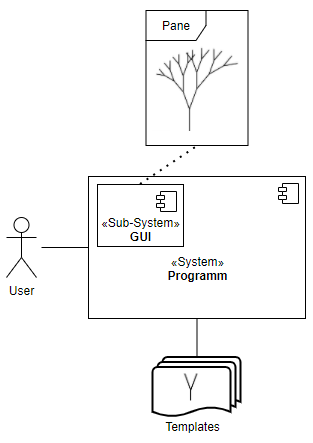
\includegraphics[width=6.2cm]{../images/Fachlicher_Kontext.PNG}
    \caption{System und Systemumgebung}
\end{figure}
\begin{figure}[H]
    \centering
    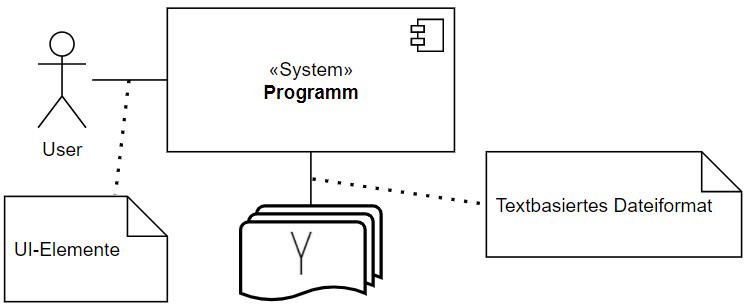
\includegraphics[width=10cm]{../images/Technischer_Kontext.PNG}
    \caption{Interaktion zwischen System und Systemumgebung}
\end{figure}

\newpage

\subsection*{Lösungsstrategie}
Zur Erreichung der o.g. Qualitätsziele werden folgende Architekuransätze umgesetzt:
\begin{center}
    \begin{tabular}{l|l}
        \textbf{Qualitätsziel} & \textbf{Architekturansatz} \\
        \hline \\
        Funktionalität &
        \begin{minipage}[t]{0.8\textwidth}
            Grafische Benutzerschnittstelle\\
            Generieren der Baumstruktur\\
            Verarbeiten von L-Systemen
        \end{minipage} \\
        \\ \hline \\
        Interoperabilität &
        \begin{minipage}[t]{0.8\textwidth}
            Durch das Nutzen allgemeingültiger mathematischer Beschreibungen sollen erstellte
            L-Systeme in Fremdsystemen, wie Online Visualisierer, genutzt werden können
        \end{minipage} \\
        \\ \hline \\
        Erweiterbarkeit &
        \begin{minipage}[t]{0.8\textwidth}
            Das Nutzen des Pipeline Design Patterns soll das Erweitern des Systems durch
            Hinzufügen weiterer Teilschritte (Pipes) erleichtern.
            Trennung der grafischen Oberfläche und der Logik durch Aufbauen des Szenengraphen über ein
            XML-Dateiformat
        \end{minipage} \\
        \\ \hline \\
        Modularität &
        \begin{minipage}[t]{0.8\textwidth}
            Sowohl eine sinnvolle Aufteilung von Funktionalitäten auf Dateien und Software-Pakete, als
            auch effiziente Datenkapselung und geschlossene Informationskontexte sorgen für Modularität des
            Programms
        \end{minipage} \\
        \\ \hline
    \end{tabular}
\end{center}

\subsection*{Bausteinsicht}
Der Benutzer interagiert über das User Interface mit dem Subsystem GUI, das sich mit der Visualisierung, dem Aufbau der
Eingabestruktur und dem Anglegen einer internen Baumtopologie beschäftigt.
Die Pipeline zum Erzeugen der Ausgabestrukturen beginnt mit dem Inferrieren eines L-Systems aus der benutzerdefinierten
Struktur und gibt das erzeuge Ersetzungssystem an die folgenden Komponenten weiter.
Hierbei gilt der Pipeline-Kontext, welcher innerhalb der Pipeline an den jeweils nächsten Schritt weitergegeben und
dort aktualisiert wird, als Eingabe der Pipeline.
Hat die Estimator-Komponente eine Verteilung über vom Benutzer angelegte Transformationsparameter angelegt, gilt
der Kontext als Ausgabe der Pipeline.

\underline{Ebene 1}
\begin{figure}[H]
    \centering
    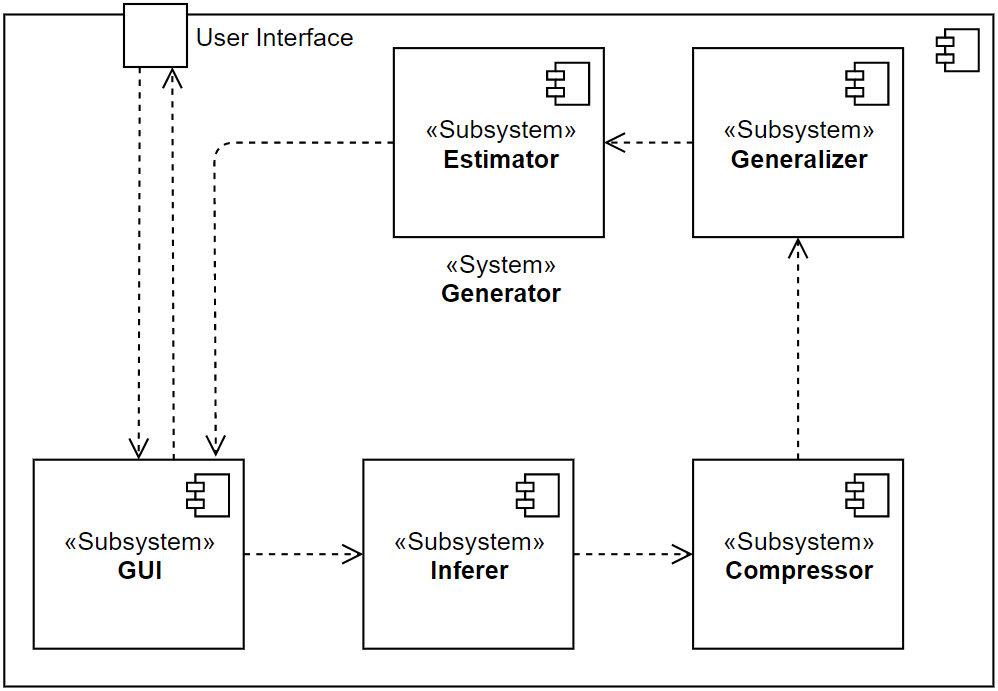
\includegraphics[width=12cm]{../images/Bausteinsicht_Ebene_1.PNG}
    \caption{Subsysteme mit fachlichen Abhängigkeiten}
\end{figure}

Betrachtet man die GUI-Komponente genauer, setzt sich diese aus vier Subsystemen zusammen.
Das Application-Modul beschreibt den Einstigspunkt für ein JavaFX-Programm.
Die grafische Benutzerschnittstelle wird über ein XML-basiertes FXML-Dateischema (Scene graph) mit zugeförigem FXML-Controller (Model)
aufgebaut.
Der Controller stellt die Logik für eine JavaFX-Oberfläche zur Verfügung.
Neben der Erstellung der Basisstruktur, wird die Baumstruktur in einer seperaten Komponente umgesetzt.

\underline{Ebene 2}
\begin{figure}[H]
    \centering
    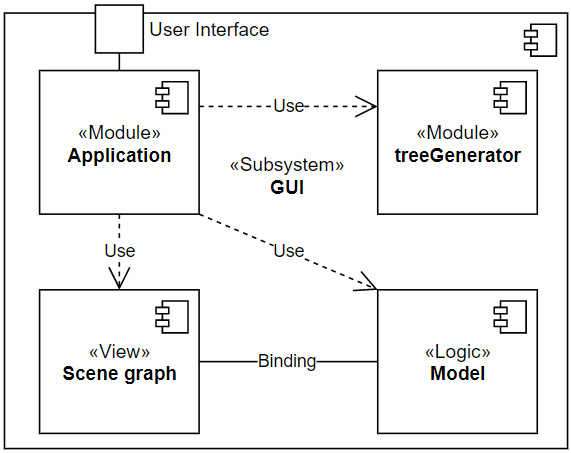
\includegraphics[width=9cm]{../images/Bausteinsicht_Ebene_2.PNG}
    \caption{Subsystem GUI}
\end{figure}

\subsection*{Laufzeitsicht}
Aus der nachfolgenden Abbildung geht hervor, wie sich der Informationsfluss zwischen den einzelnen Subsystemen verhält.
Wird der Systemprozess einmal durchlaufen, besteht die Möglichkeit die Ausführung des generalisierten L-Systems mit
erneuter Vergabe der Transformationsparameter aus der Häufigkeitsverteilung der Estimator-Komponente zu starten.
Der Ablauf des Systems setzt sich wie folgt zusammen:

\begin{figure}[H]
    \centering
    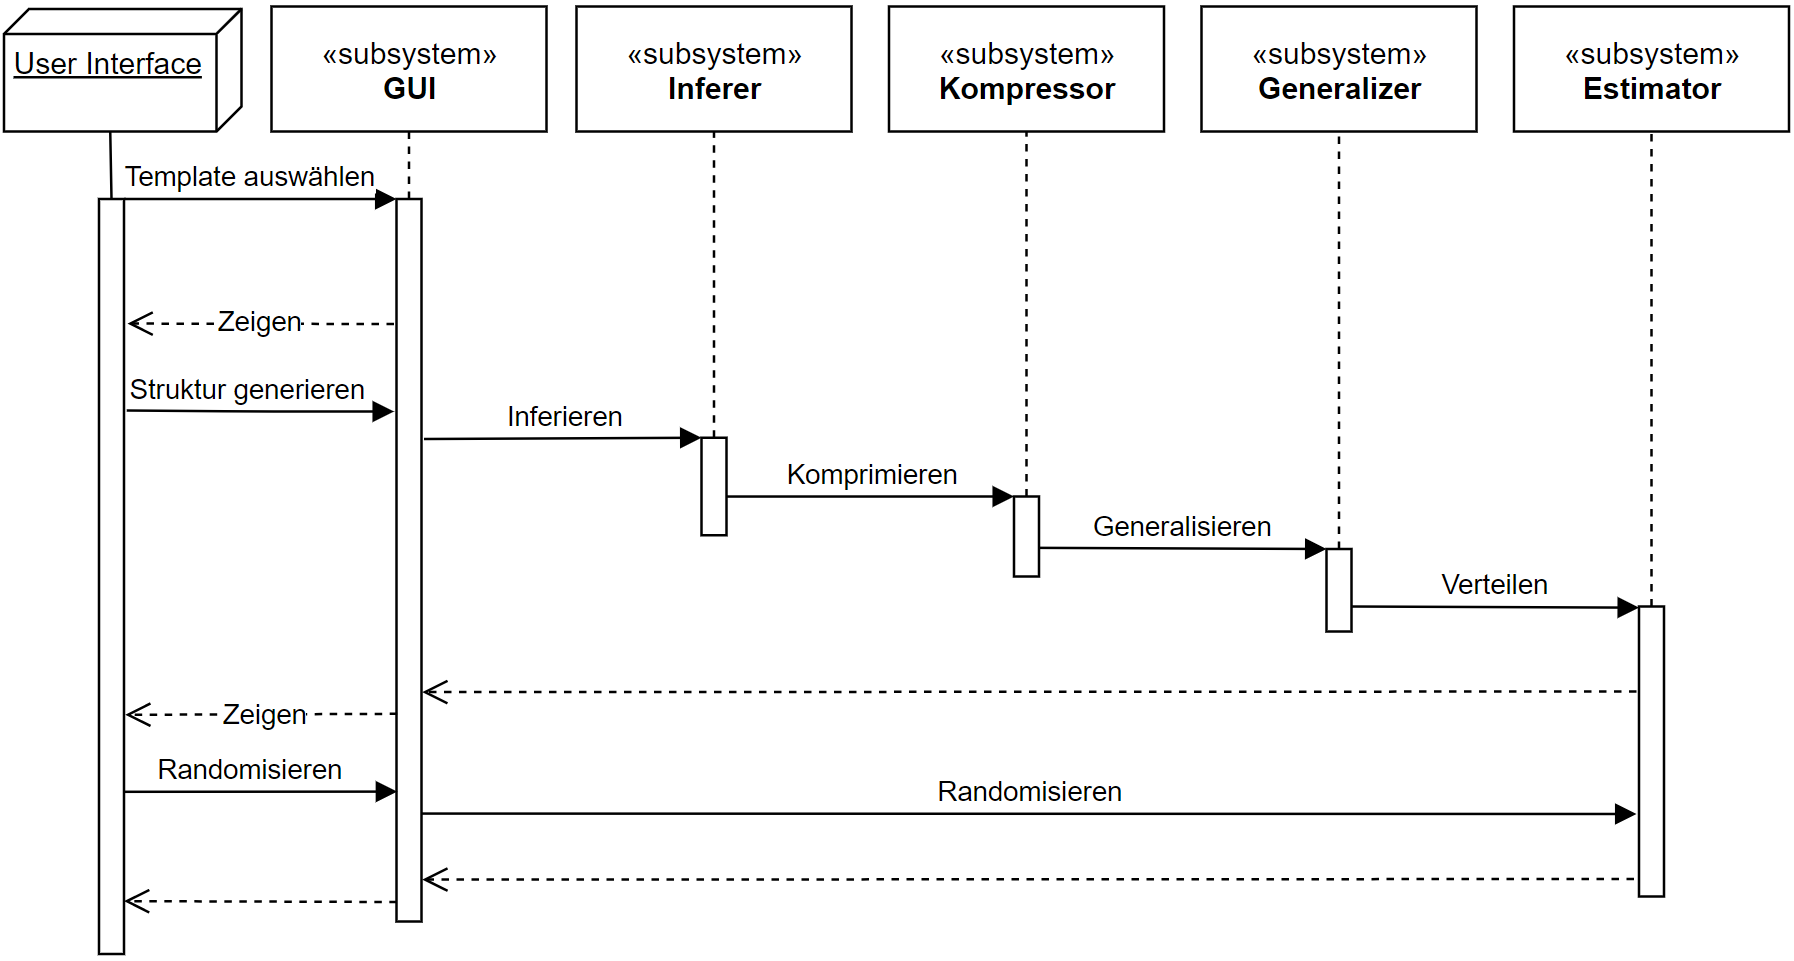
\includegraphics[width=14cm]{../images/Laufzeitsicht.PNG}
    \caption{Laufzeitsicht}
\end{figure}

\subsection*{Verteilungsicht}
Die Ausführung des Programms wird durch ein einfaches Startskript zur Verfügung gestellt.
Die folgende Abbildung der Verteilungssicht stellt lediglich die Ausführung auf einer Windows-Maschine dar.

\begin{figure}[H]
    \centering
    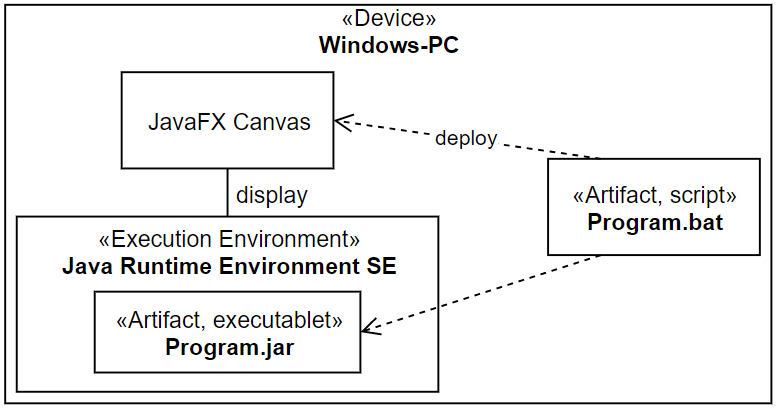
\includegraphics[width=10cm]{../images/Verteilungssicht.PNG}
    \caption{Infrastruktur Windows-PC}
\end{figure}

\subsection{Weitere Konzepte}

\subsubsection{Testbarkeit}
Um eine ausreichende Testabdeckung zu erreichen, werden Klassen als kleinstmöglich zu testende Einheit definiert
und durch Komponententests geprüft.
Der Name eines Tests setzt sich aus dem Präfix als Name der zu testenden Klasse oder Releases und dem Suffix
"`Test"'
zusammen.
Testsubjekte werden als \textbf{Blackbox} behandelt, also anhand der Spezifikation getestet.
\begin{center}
    Bsp.: Klasse \textit{Inferer} mit Komponententest \textit{InfererTest}
\end{center}
Da jedes Release der Implementierung ein funktionsfähiges System beinhaltet, kann auf Integrationstests
verzichtet werden.
Weiter wird ein Release anhand von funktionalen und nicht-funktionalen Anforderungen getestet.
Anhand dieser Systemtests wird geprüft, ob Gesamtspezifikationen umgesetzt worden sind.
\begin{center}
    Bsp.: Release 2 mit Systemtest \textit{Release2Test}
\end{center}
Zum Schluss der Implementierung wird ein Akzeptanztest durchgeführt.

\subsubsection{Validierung}
Der Benutzer des Systems nutzt eine grafische Schnittstelle.
Somit kann sichergestellt werden, dass dieser keine ungültigen Eingaben tätigt.
Werden Template-Dateien unter einem bestimmten Dateipfad nicht gefunden, wird eine \textit{NotFound}-Exception
protokolliert und dem Benutzer eine Nachricht über ein Pop-up mitgeteilt.
Eine \textit{IllegalArgumentException} wird verzeichnet und ausgegeben, wenn eingelesene Template-Dateien
strukturelle Fehler aufweisen.

\subsubsection{Fehlerbehandlung}
Zur Fehlersuche und -behandlung biete sich eine Protokollierung über Vorgänge, Fehler und Ausnahmen an.
Bestimmte Fehler werden dem Benutzer weitergegeben und grafisch angezeigt.
Folgende Subsysteme werden in das Programm integriert:
\begin{itemize}
    \item Ausnahmebehandlung (Exception Handling) und
    \item Protokollierung (Logging)
\end{itemize}
Erwartete Exceptions werden jeweils mit eigenen Klassen abgebildet, die von einer entsprechenden Klasse aus der
Exception-Hierarchie abgeleitet sind.
Das Logging ist statisch und überall im System zugreifbar, um eine einheitliche Protokollierung zu gewährleisten.

\subsection{Datenstrukturen}
TODO: Klassendiagramm aus IntelliJ generieren
% @author Arian Helberg

\chapter{Implementierung}

Zur Umsetzung der vorgestellten Konzepte wird im Folgenden auf Softwarepakete, Technologien, Datenspeicherung,
Benutzerinteraktion und Arbeitsablauf der erstellten Software eingegangen.
Darüber hinaus wird ein Überblick über genutzte Hardware und einige Implementierungsentscheidungen gegeben.
Auf Implementierungsdetails zur Nutzung der vorgestellten Technologien wird nicht eingegangen.

\section{Projektstruktur}
Das Softwareprojekt ist nach der Gradle-Source-Code-Konvention organisiert.
Das gesamte Programm befindet sich im Ordner Generator, der obligatorische Gradle-Dateien und den
Source-Ordner enthält.
Sowohl die Quelldateien, also auch die Testdateien sind der Paketstruktur \textbf{de.haw} untergeordnet.
Die folgende Tabelle gibt einen Überblick über grundlegende Pakete und deren Funktion.

\begin{figure}[H]
    \centering
    \begin{tikzpicture}
        \draw[color=black!60!white]
        \FTdir(\FTroot,root,Generator){
            ++(0,-0.2em)
            \FTdir(root,src,src){
                ++(0,-0.2em)
                \FTdir(src,main,main){
                    ++(0,-0.2em)
                    \FTdir(main,java,java) {
                        ++(0,-0.2em)
                        \FTdir(java,de,de) {
                            ++(0,-0.2em)
                            \FTdir(de,haw,haw) {
                                ++(0,-0.5em)
                                \FTdir(haw,gui,gui) {
                                    ++(0,-0.5em)
                                    \FTdir(gui,shape,shape) {}
                                    ++(0,-0.5em)
                                    \FTdir(gui,structure,structure) {}
                                    ++(0,-0.5em)
                                    \FTdir(gui,template,template) {}
                                    ++(0,-0.5em)
                                    \FTdir(gui,turtle,turtle) {}
                                }
                                ++(0,-0.5em)
                                \FTdir(haw,lsystem,lsystem) {}
                                ++(0,-0.5em)
                                \FTdir(haw,pipeline,pipeline) {
                                    ++(0,-0.5em)
                                    \FTdir(pipeline,pipe,pipe) {}
                                }
                                ++(0,-0.5em)
                                \FTdir(haw,tool,tool) {}
                                ++(0,-0.5em)
                                \FTdir(haw,tree,tree) {}
                                ++(0,-0.5em)
                                \FTdir(haw,tree,utils) {}
                            }
                        }
                    }
                }

                \FTdir(src,test,test) {
                    \FTdir(test,java,java) {
                        \FTdir(java,de,de)
                    }
                }
            }
        };
    \end{tikzpicture}
    \caption{Softwareprojekt Dateistruktur}
\end{figure}

\begin{figure}[H]
    \centering
    \begin{tabular}{l|l}
        \textbf{Paket} &  \textbf{Funktion} \\ \hline
        \textit{gui} & Visualisierung des Programms \\ \hline
        \textit{lsystem} & L-System-Repräsentation \\ \hline
        \textit{pipeline} & Umsetzung des Pipeline-Design-Patterns \\ \hline
        \textit{tool} & Methodiken und Algorithmen \\ \hline
        \textit{tree} & Komponenten der Baumstruktur \\ \hline
        \textit{utils} & Hilfskomponenten
    \end{tabular}
    \caption{Softwarepakete mit zugehörigen Funktionen}
\end{figure}

\section{Technologien}
Zur Umsetzung des Softwarepojektes wird eine Java-Anwendung für die Java-Laufzeitumgebung entwickelt.
Sie liegt in der Distribution \textbf{Amazon Corretto} in der Version 11.0.3\_7 vor.
Grafische Oberflächen werden mit der JavaFX-Spezifikation von Oracle in der Version 11.0.2 umgesetzt.
Zur Automatisierung von Abhängigkeits- und Buildmanagement wird Gradle (Version 6.7) verwendet.
Eine Testumgebung, eine Vektorbibliothek, eine Tupelrepräsentation und eine Erweiterung zur mathematischen
Standartbibliothek werden über Abhängigkeiten vom Gradle-Framework im Build-Prozess geladen und zur Verfügung
gestellt.\\
Um den test-driven Implementierungsansatz umzusetzen wird JUnit 5 Jupiter als Testumgebung genutzt.
Sie setzt sich aus einem Programmierschema und einem Erweiterungsmodell zusammen.
Das Jupiter-Projekt liefert zudem die Laufzeitumgebung für Softwaretests.
Googles Guava liefert eine Bibliothek mit mathematischen Funktionen.
Sie wird benötigt, um eine praktikable Lösung zu Mengenmanipulation nutzen zu können (Bsp. Erstellen
von Kombinationspaaren einer Menge).
Ausschließlich JavaFX wird außerhalb des Projektes installiert und als Modul im Start-Skript des Programmes
hinzugefügt.
\\~\\
Weitere Systeme zur Erstellung des Softwareprojektes sind:
\begin{itemize}
    \item Versionierung via Git,
    \item Dot zur Visualisierung von Graphen und
    \item PlantUML zur Generierung von UML-Diagrammen
\end{itemize}

\section{Konzeptumsetzung}

Das Skript \texttt{Generator.bat}, das zum Starten der Anwendung innerhalb eines Windows-Betriebssystems genutzt werden kann,
fügt dem Programm alle externen Module hinzu, die während der Laufzeit genutzt werden, und führt die angegebene jar-Datei aus:
\begin{figure}[H]
    \centering
    \begin{csource}
        java --module-path .\javafx-sdk-11.0.2\lib --add-modules javafx.controls,javafx.fxml,javafx.graphics -jar Generator-0.1.jar
        pause
    \end{csource}
    \caption{Startskript Generator.bat}
\end{figure}

Beim Start der Anwendung findet der Benutzer die grafische Oberfläche vor.
\begin{figure}[H]
    \centering
    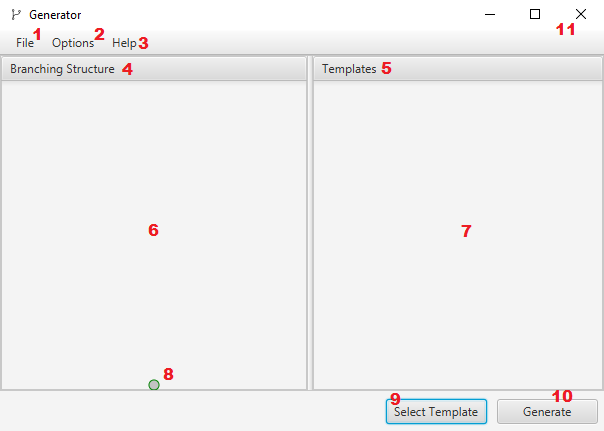
\includegraphics[width=14cm]{../images/UI_numbers.png}
    \caption{Programm nach Ausführung des Start-Skripts}
\end{figure}
Der Menüeintrag \textbf{1} bietet Funktionen zum Öffnen des Dateipfades und zum Laden der angelegten Templates-Datei.
\textbf{2} dient zur Konfiguration der Umgebungsparameter für die Anzahl Iterationen der Ausführung
und die Anzahl an Ähnlichkeitsstrukturen, die aus dem resultierenden L-System abgeleitet werden können.
Die Gewichtungsparameter der vorgestellten Algorithmen können ebenfalls hier eingestellt werden.
Die Hilfe (\textbf{3}) gibt Informationen zum Projektkontext und zur Benutzung der Anwendung.
Die Strukturen \textbf{4} und \textbf{5} gliedern das Programm in die Ansicht der Verzweiungsstruktur (\textbf{6}), die vom Benutzer
angelegt wird, die Übersicht zur Auswahl eines Templates (\textbf{7}) und eine Sicht zur Setzung von Transformationsparametern (\textbf{7}).
Der Kreis \textbf{8} stellt einen Anker dar, an welchen eine Template-Instanz angehängt werden kann.
Sowohl über einen Doppelklick, also auch über einen Button (\textbf{9}) kann ein Template aus der Tempalte-Liste (\textbf{7})
ausgewählt werden.
Ist die Verzweigungsstruktur vom Benutzer fertiggestellt, kann die Synthese zur Erstellung der Ähnlichkeitsabbildungen
mit \textbf{10} erfolgen.
\textbf{11} schließt die Anwendung.

\subsection*{Visualisierung}

Die grafische Oberfläche liegt als MVC-Pattern in Form des Application State (Model), der XML-basierten FXML-Datei (View)
und dem JavaFX-Controller vor.
Der Arbeitsablauf zur Erstellung der Verzweigungsstruktur kann Schritt für Schritt umgesetzt werden, nachdem die Templates
geladen wurden.
Dies wird an folgendem Beispiel deutlich gemacht.
Die Parameter \textbf{Number of iterations}, \textbf{Number of generations}, \textbf{Rule application ratio} und
\textbf{Merge application ratio} werden auf die Werte \textbf{8}, \textbf{5}, \textbf{0.5} und \textbf{0.5} gesetzt
(Standarteinstellung).
\begin{figure}[H]
    \centering
    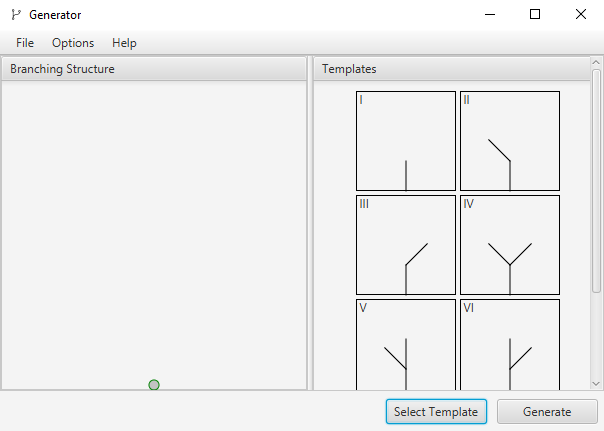
\includegraphics[width=7cm]{../images/UI_templates.png}
    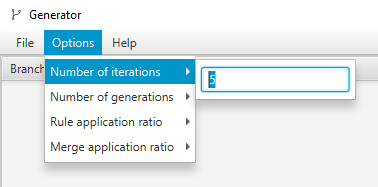
\includegraphics[width=7cm]{../images/UI_parameters.png}
    \caption{Erster Anker ist vorselektiert \& gesetzte Parameter}
\end{figure}

\begin{figure}[H]
    \centering
    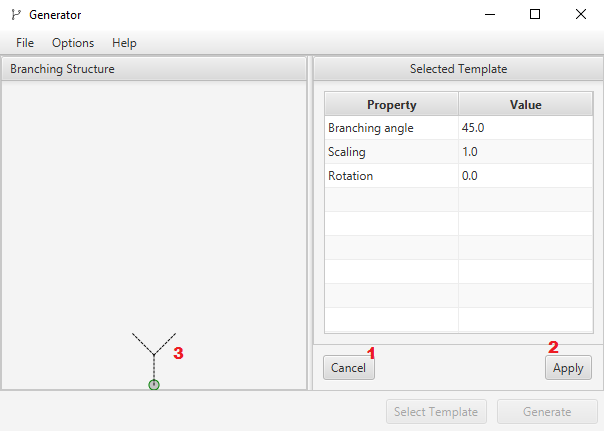
\includegraphics[width=12cm]{../images/UI_template.png}
    \caption{Auswahl des ersten Templates}
\end{figure}

Nachdem ein Template ausgewählt wurde, können die Transformationsparameter gesetzt (Doppelklick) werden und die Auswahl
rückgängig gemacht (\textbf{1}) oder bestätigt (\textbf{2}) werden.
\textbf{3} zeigt einen Entwurf der Tempalte-Instanz, die mit den aktuellen Transformationsparametern angepasst wurde.
Mit der Bestätigung wird die Template-Instanz endgültig der Basisstruktur hinzugefügt und der Benutzer gelangt wieder
in die Übersich der zur Verfügung stehenden Templates.
\begin{figure}[H]
    \centering
    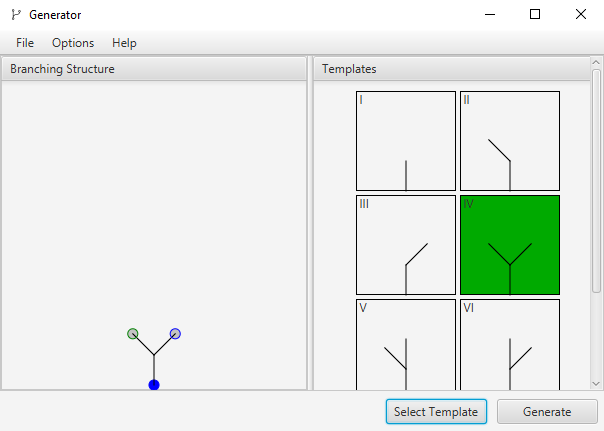
\includegraphics[width=12cm]{../images/UI_applied.png}
    \caption{Der Verzweigungsstruktur hinzugefügte Template-Instanz}
\end{figure}

Dieser Vorgang wiederholt sich, bis der Benutzer die Struktur fertiggestellt hat.
\begin{figure}[H]
    \centering
    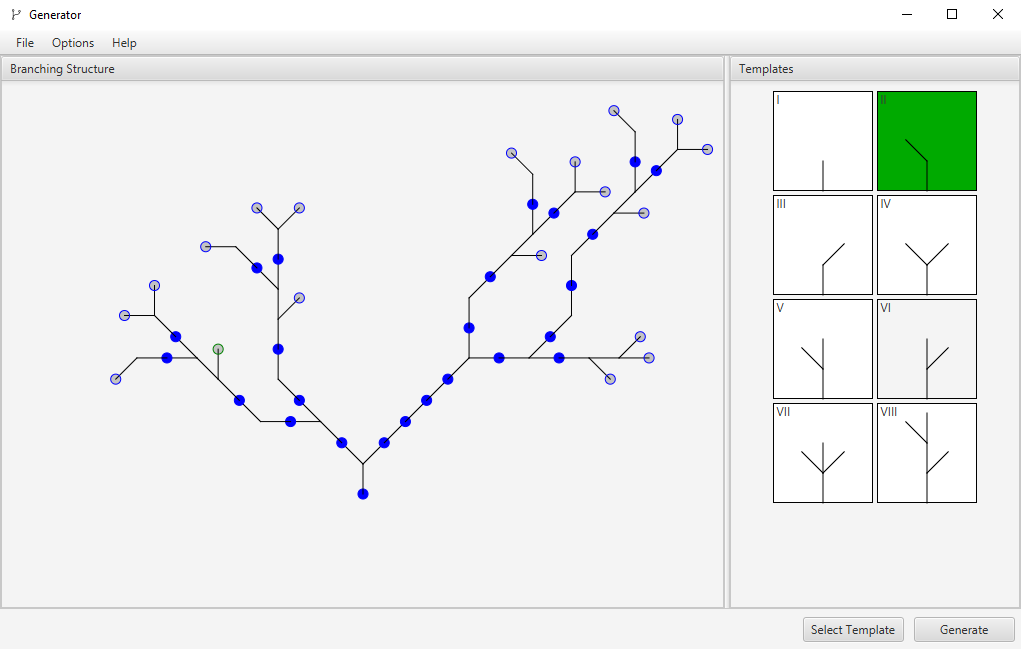
\includegraphics[width=13cm]{../images/UI_finished.png}
    \caption{Vom Benutzer fertiggestellte Verzweigungsstruktur}
\end{figure}

Über den \textbf{Generate}-Button kann nun die Synthese gestartet werden.
Es ergeben sich 5 (\textbf{Number of generations}) Ähnlichkeitsstrukturen

\begin{figure}[H]
    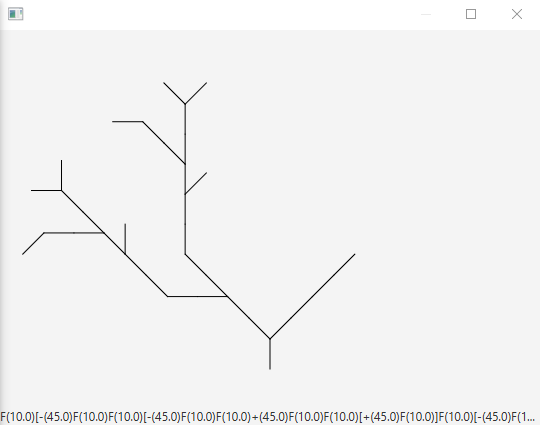
\includegraphics[width=6cm]{../images/example_1.png}
    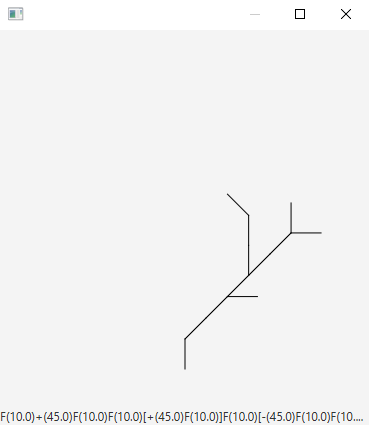
\includegraphics[width=6cm]{../images/example_2.png}
    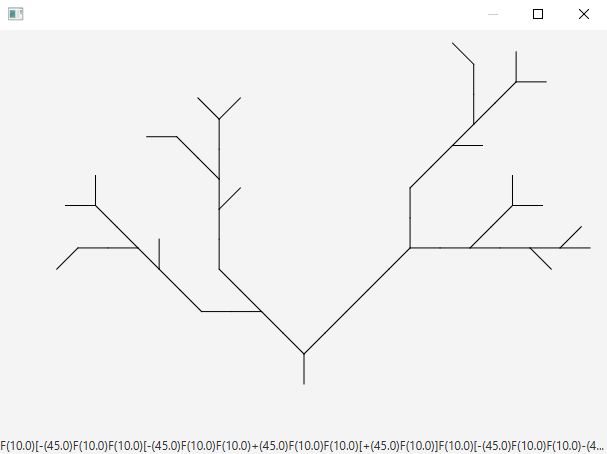
\includegraphics[width=6cm]{../images/example_3.png}
    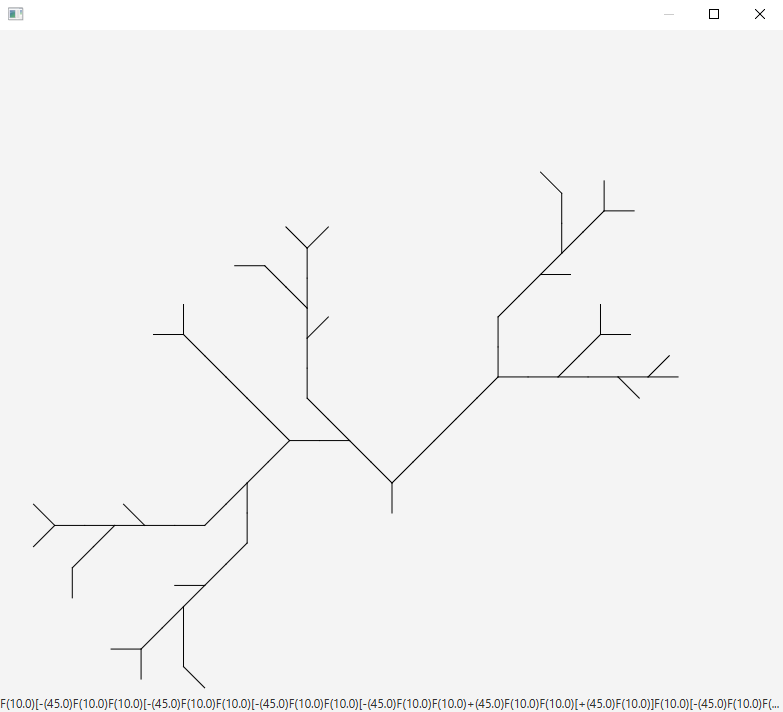
\includegraphics[width=6cm]{../images/example_4.png}
    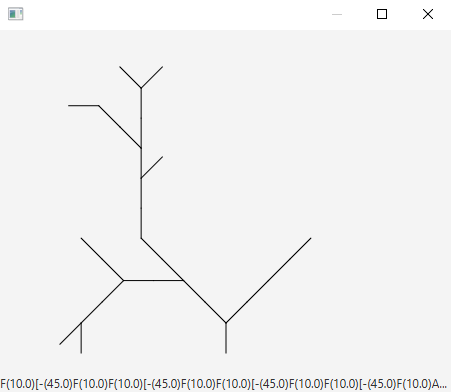
\includegraphics[width=6cm]{../images/example_5.png}
    \caption{Generierte Verzweigungsstrukturen}
\end{figure}

\subsection*{Baumtopologie}
Um eine interne Baumtopologie aufzubauen wird die Klasse \texttt{TreeNode} verwendet, um eine iterierbare Baumstruktur
aufzubauen:
\begin{lstlisting}[
    basicstyle=\footnotesize,
    commentstyle=\color{comment},
    keywordstyle=\color{orange},
    language=Java,
    numberstyle=\color{gray}
]
/**
 * Iterable tree node structure containing a payload and children
 * as tree nodes.
 * Every node represents a whole tree
 * @param <T> Tree node content
 */
public class TreeNode<T> implements Iterable<TreeNode<T>> {
    // Payload
    private T data;
    // Children
    protected List<TreeNode<T>> children;
    ...
    @Override
    public Iterator<TreeNode<T>> iterator() {
        return new TreeNodeIterator<>(this);
    }
    ...
}
\end{lstlisting}

\texttt{TreeNode} implementiert die \texttt{Iterable}-Schnittstelle, was ein Überladen der \texttt{iterator}-Funktion möglich
macht.
Sie stellt einen Iterator des Baumes zur Verfügung.
Dieser Iterator (\texttt{TreeNodeIterator}) implementiert die \texttt{Iterator}-Schnittstelle und definiert so die Funktionen
\texttt{hasNext} und \texttt{next}.
\begin{lstlisting}[
    basicstyle=\footnotesize,
    commentstyle=\color{comment},
    keywordstyle=\color{orange},
    language=Java,
    numberstyle=\color{gray}
]
/**
 * Tree node iterator for iterating nodes of a tree
 * @param <T> Payload of the tree nodes
 */
public class TreeNodeIterator<T> implements Iterator<TreeNode<T>>{
    ...
    @Override
    public boolean hasNext() {
        return !queue.isEmpty();
    }

    @Override
    public TreeNode<T> next() {
        if (queue.isEmpty()) return null;
        var node = queue.pop();
        queue.addAll(node.getChildren());
        return node;
    }
}
\end{lstlisting}
Die Funktion \texttt{next} zeigt, wie eine Iteration des Baumes als Breitensuch e implementiert ist.
Diese wird beim Inferrieren eines L-Systems aus der Baumstruktur benötigt.
Das folgende Beispiel zeigt eine erstellte Baumstruktur (links) und deren erstellte Baumtopologie (rechts).
\begin{figure}[H]
    \centering
    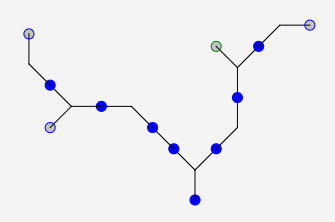
\includegraphics[width=8cm]{../images/graph_tree.png}
    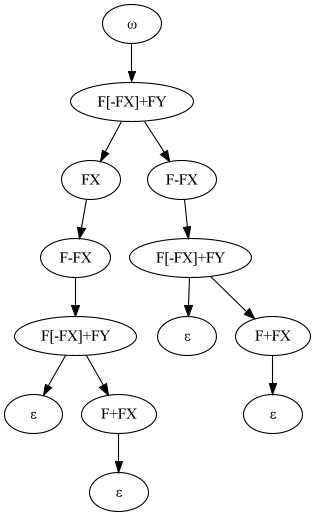
\includegraphics[width=5cm]{../images/tree_graph.png}
    \caption{Verzweigungsstruktur \& zugehörige Baumstruktur}
\end{figure}

\subsection*{Prozesspipeline}



\section{Entscheidungen}

\subsection*{Änderbarkeit}
\subsection*{Risiken}
\subsection*{Qualitätsmerkmale}
\subsection*{Alternativen}
\subsection*{Aufwand der Implementierung}
% @author Arian Helberg

\chapter{Evaluierung}
Die Synthese von Verzweigungstrukturen wird in den vorangegangenen Kapiteln konzeptionell betrachtet
und in einem Softwareprojekt umgesetzt.
Im Folgendem werden Teilaspekte an einem fortlaufenden Beispiel evaluiert und bewertet.
Diese Aspekte umfassen
\begin{itemize}
    \item das Nutzen von Templates
    \item die Erstellung und Visualisierung von Verzweigungsstrukturen
    \item Aufbau einer Baumstruktur
    \item Extrahierung von Regeln und Mustern
    \item Komprimierung von L-Systemen
    \item Erweitern von L-Systemen
    \item Synthese der Ähnlichkeitsstrukturen
    \item Auswirkung der Gewichtungsparameter
\end{itemize}

\subsection*{Templates}
Die Nutzung von Templates als Terminale einer Grammatik findet Anwendung in vielen wissenschaftlichen Arbeiten.
\citeauthor{aliaga_2016} liefert hierzu eine umfassende Übersicht~\cite{aliaga_2016}.
Mit der Verwendung einer allgemeinen Repräsentation mithilfe von \textit{turtle}-Befehlen, wird eine
Wiederverwendbarkeit der genutzten Templates sichergestellt.
Die in dieser Arbeit erstellte Software nutzt ein minimalistisches System zum Einlesen der Templates aus
einer textbasierten Datei, während die Forschung zur inversen prozeduralen Modellierung den Einsatz von
neuronalen Netzen als vielversprechende Methode Strukturen zu erkennen und Regeln abzuleiten, zeigt.\\
Während neuronale Netze eine Eingabestruktur analysieren und in einer baumähnlichen Struktur organisieren,
knüpft diese Arbeit hier an und nutzt stattdessen aus Praktikabilitätsgründen eine benutzergeführte Anordnung
von Templates zu einer Verzweigungsstruktur.\\~\\
\underline{Beispiel}: Die Template-Zeichenketten haben folgende Form:
\begin{figure}[H]
    \centering
    \begin{csource}
FX
F-FX
F+FX
F[-FX]+FY
F[-FX]FY
F[FX]+FY
F[-FX][FY]+FZ
F[+FX]F[-FY]FZ
    \end{csource}
    \caption{templates.txt}
\end{figure}
\textit{F}, \textit{-}, \textit{+}, \textit{[} und \textit{]} sind dem Turtle-Algorithmus bekannte
Befehlssymbole.
Alle anderen Symbole (z.B. \textit{X, Y, Z}) stellen Verzweigungsvariablen dar, um anzuzeigen, an welcher Stelle
der Templatestruktur eine neue Verzweigung abgehen kann.

\subsection*{Erstellung und Visualisierung}
Durch die Ausführung bestimmter \textit{turtle}-Befehle der template-basierten Struktur, wird diese visualisiert.
Darum bietet es sich an, einfache grafische Elemente zu nutzen, um Verzweigungsstrukturen sichtbar zu machen
(z.B. Canvas).
Das Programm nutzt stattdessen interaktive Elemente innerhalb eines JavaFX Pane gegenüber staatischen Elementen, um
die Strukturen zu zeichnen, da der Prozess der Erstellung benutzergeführt und damit interagierbar sein muss.
So können Elemente genutzt werden, mit denen der Benutzer kommunizieren kann (z.B. klickbare Kreise).
Es ist nun möglich Verzweigungsstrukturen in einem simplen Arbeitsablauf zu ertstellen.

\newpage

\underline{Beispiel}: Aus der Erstellung der Verzweigungsstruktur ergibt sich:
\begin{figure}[H]
    \centering
    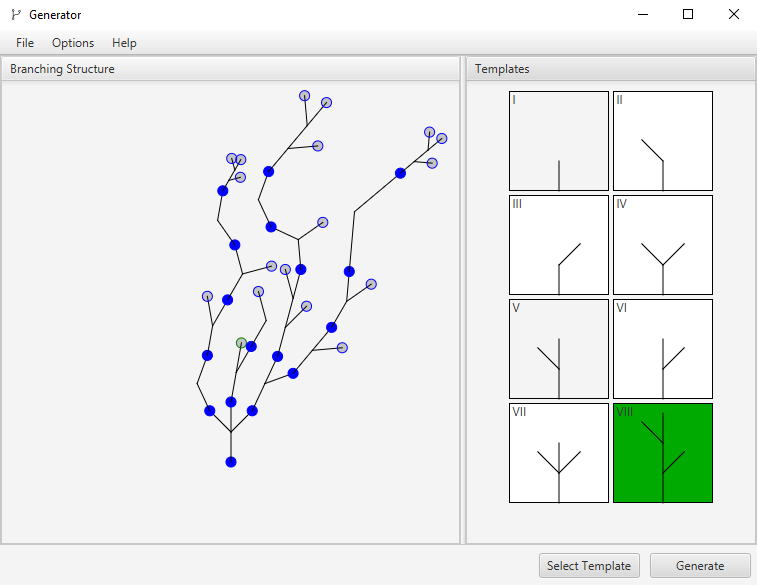
\includegraphics[width=12cm]{../images/evaluierung_inferrieren.png}
    \caption{Grafische Benutzeroberfläche nach der Erstellung einer Basisstruktur}
\end{figure}

\subsection*{Aufbau einer Baumstruktur}
Baumähnliche Strukturen eignen sich gut, um Tansformationsparameter und topologische Anordnung von Tempaltes
datenstrukturell zu trennen.
Ansätze zur ganzheitlichen Betrachtung von Eingabestrukturen, also das Einbinden der Transformationen,
und zur Trennung von Transformation und Topologie sind Gegenstand der Forschung.
Das von \citeauthor{benes_2011} vorgestellte System nutz beispielsweise einen ganzheitlichen Ansatz, um sog.
\textit{Guides} zu erstellen, welche Teilsysteme der Eingabestruktur beschreiben.
Hier unterscheiden sich Strukturen, die zwar identische Verzweigungen aufweisen, sich aber in Ausprägungen
von Transformationsparametern (z.B. der Winkel von Verzweigungen) voneinander entfernen.
Auch in der Arbeit~\cite{stava_2010} von \citeauthor{stava_2010} zeigt sich eine Organisation von
"`Clustern"' mit Transformationen, die in eine Signifikanzbewertung einfließen.

\newpage

Auf der anderen Seite zeigen \citeauthor{nishida_2016} und \citeauthor{guo_2020},
dass zum Einen eine seperate Untersuchung der Transformationen mithilfe eines zweiten,
auf seine Aktivität zugeschnittenes, neuronales Netz~\cite{nishida_2016}, zum Anderen, dass die meisten
räumlichen Transformationen die Erkennung mittels neuronalem Netz nicht signifikant beeinflussen,
sinnvoll ist.\\~\\
Diese Arbeit legt der Fokus auf die datenstrukturelle Trennung von Transformationen und topologischer
Anordnung und erstellt somit eine Baumstruktur, die Template-Instanzen als Knoten und
räumliche Transformationen als eingehende Kanten darstellt.\\~\\
\underline{Beispiel}: Aus der Eingabestruktur ergibt sich folgender Baum (die räumlichen Transformationen,
die die eingehenden Kanten jedes Knotens darstellen, sind hier nicht visualisiert):
\begin{figure}[H]
    \centering
    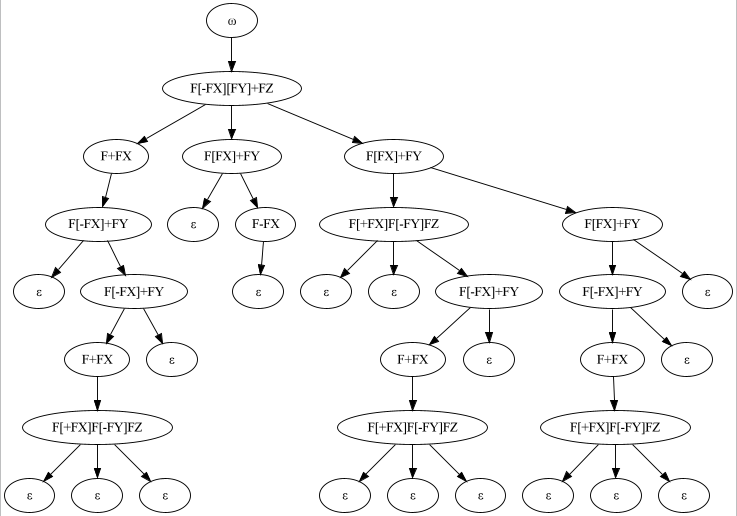
\includegraphics[width=12cm]{../images/evaluierung_inferrieren_baum.png}
    \caption{Baumstruktur der erstellten Verzweigungsstruktur}
\end{figure}

\subsection*{Extrahieren von Regeln und Mustern}
Die in~\ref{alg2} vorgestellte Methodik zum Inferieren eines L-Systems aus einer Baumstruktur
stellt einen Algorithmus vor, der auf die spezielle Baumstruktur zugeschnitten ist.
Die L-Systeme entsprechen lediglich der Eingabestruktur und beinhalten keine Transformationen.\\~\\
\underline{Beispiel}: Ausgeführte Ersetzungssysteme werden über einen JavaFX Dialog visualisiert:
\begin{figure}[H]
    \centering
    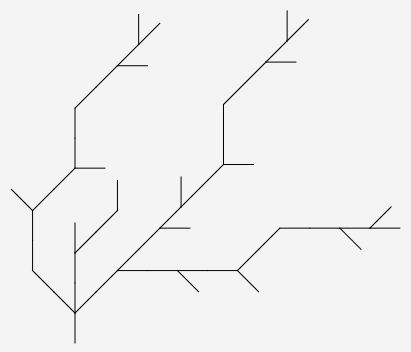
\includegraphics[width=8cm]{../images/evaluierung_inferrieren_lsystem.png}
    \caption{Inferriertes L-System}
\end{figure}
Die Zeichenkettenrepräsentation des L-Systems ($\mathcal{L}=\{M,\omega,R\}$) lautet:
\begin{csource}
LSystem{
    [F, S, A, B, C, D, E, G, H, I, J, K, L, M, N, O, P, Q, R, T, U, V, W, X, Y, Z, a, b, c, d, e, f, g, h, i, j, k],
    S,
    [S -> A, A -> F[-FB][FC]+FD, B -> F+FE, C -> F[FG]+FH, D -> F[FI]+FJ, E -> F[-FK]+FL, G -> _, H -> F-FM, I -> F[+FN]F[-FO]FP, J -> F[FQ]+FR, K -> _, L -> F[-FT]+FU, M -> _, N -> _, O -> _, P -> F[-FV]+FW, Q -> F[-FX]+FY, R -> _, T -> F+FZ, U -> _, V -> F+Fa, W -> _, X -> F+Fb, Y -> _, Z -> F[+Fc]F[-Fd]Fe, a -> F[+Ff]F[-Fg]Fh, b -> F[+Fi]F[-Fj]Fk, c -> _, d -> _, e -> _, f -> _, g -> _, h -> _, i -> _, j -> _, k -> _]
}
\end{csource}

Das inferrierte L-System zeigt, dass die Eingabestruktur richtig in eine Grammatik überführt wurde.
Dabei steht der Unterstrich (\_) für das leere Wort $\varepsilon$ und damit für die leeren Knoten
der aufgebauten Baumstruktur.

\subsection*{Komprimieren des L-Systems}
Die Zeichenkettenrepräsentation des inferrierten L-Systems zeigt einige Redundanzen auf.
Zum Beispiel bilden
\begin{csource}
P -> F[-FF+FF[+F]F[-F]F]+F
\end{csource}
und
\begin{csource}
Q -> F[-FF+FF[+F]F[-F]F]+F
\end{csource}
das gleiche Muster.
Um solche Redundanzen zu entfernen, wird das L-System in der vorgestellten Komprimierungs-Pipe reduziert.
Hierbei werden identische, maximale Unterbäume und deren leere Kindknoten zusammengefasst.
Der Gewichtungsparameter für das Beispiel wird auf 0.5 gesetzt.
Es ergibt sich folgender Baum:
\begin{figure}[H]
    \centering
    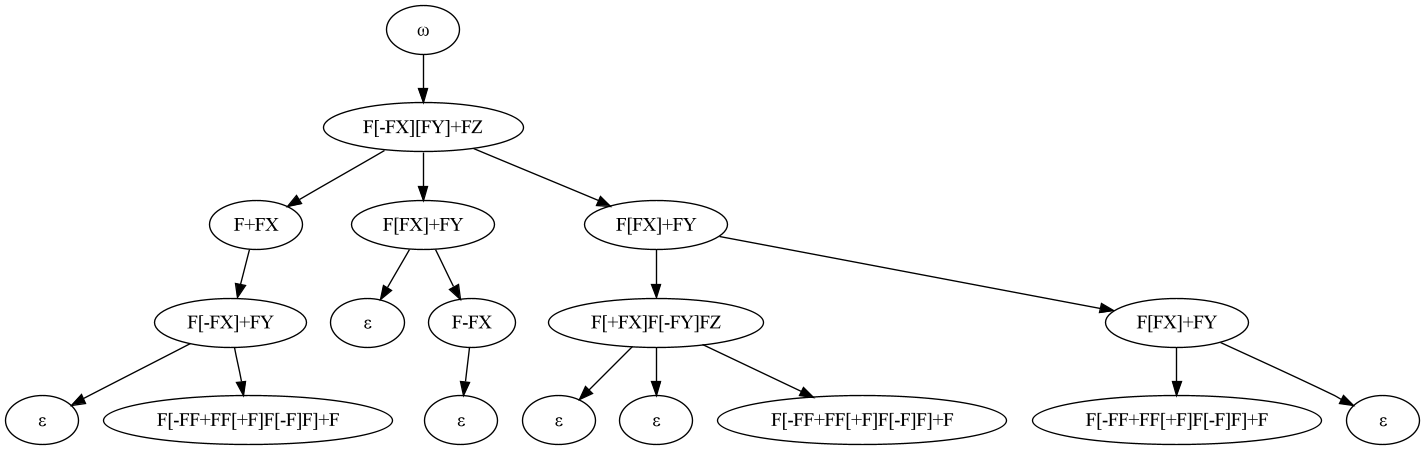
\includegraphics[width=14cm]{../images/compressed_tree.png}
    \caption{Komprimierter Baum}
\end{figure}

Die Baumstruktur zeigt, dass der Komprimierungsalgorithmus die maximalen Subbäume erfolgreich reduziert.
Das komprimierte L-System setzt sich wie folgt zusammen:
\begin{csource}
LSystem{
    [F, S, A, B, C, D, E, G, H, I, J, K, L, M, N, O, P],
    S,
    [S -> A, A -> F[-FB][FC]+FD, B -> F+FE, C -> F[FG]+FH, D -> F[FI]+FJ, E -> F[-FK]+FL, G -> _, H -> F-FM, I -> F[+FN]F[-FO]FP, J -> F[FL]+FG, K -> _, L -> F[-FF+FF[+F]F[-F]F]+F, M -> _, N -> _, O -> _, P -> F[-FF+FF[+F]F[-F]F]+F]
}
\end{csource}

\subsection*{Generalisieren des L-Systems}
Der vorgestellte Generalisierungsalgorithmus setzt das L-System von der Eingabestruktur ab, in dem
Produktionsregeln miteinander verbunden und mit einer Wahrscheinlichkeit versehen werden.
Der Gewichtungsparameter wird für das Beispiel auf 0.5 gesetzt.
Es ergibt sich das finale L-System:
\begin{csource}
LSystem{
    [F, S, E, G, K, M, N, A],
    S,
    [S -> A, E -> F[-FK]+FA, G -> _, K -> _, M -> _, N -> _, A -> F-FM, A -> F[-FA][FA]+FA, A -> F[FG]+FA, A -> F[FA]+FG, A -> F+FE, A -> F[+FN]F[-FA]FA, A -> F[-FF+FF[+F]F[-F]F]+F, A -> F[FA]+FA, A -> _]
}
\end{csource}

Die Produktionsregelmenge zeigt einige Regeln auf, die dasselbe Ziel haben.
Sie werden bei ihrer Anwendung zufällig ausgewählt.


\subsection*{Synthese}
Führt man das generalisierte L-System aus, ergeben sich die Ähnlichkeitsstrukturen.
Eine Evaluierung wird stichprobenartig durchgeführt, erweist sich aber als schwierig, da
es bei der Erstellung der Ausgabestrukturen um Wahrscheinlichkeiten beim Auftreten gewisser
Muster handelt.
Da die Algorithmen eine akzeptable Lösung eines schwierigen Problems liefern sollen,
ist die Bewertung der Ergebnisse subjektiv.
\begin{figure}[H]
    \centering
    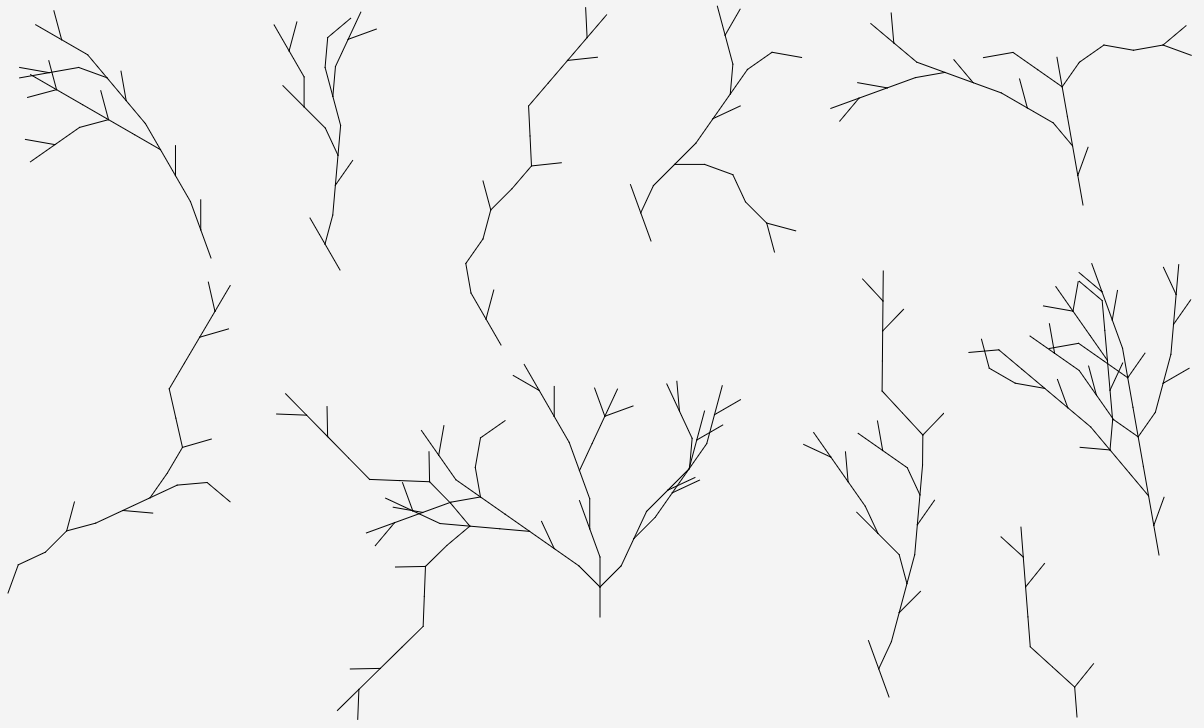
\includegraphics[width=14.5cm]{../images/synthesis.png}
    \caption{Synthetisierte Verzweigungsstrukturen}
\end{figure}

Vergleicht man die Eingabestruktur mit den synthetisierten Strukturen, weisen diese
gewisse Eigenschaften auf (siehe folgende Abbildung):
\begin{itemize}
    \item Wiederholtes Auftreten einer Struktur, die beim Synthetisieren als maximaler Unterbaum
    erkannt wurde (rot)
    \item Anwendung von benutzerdefinierten Transformationsparametern (blau)
    \item Ähnliche Häufigkeiten (grün)
    \item Isoliertes Auftreten von Templates des maximalen Subbaums,die über den Unterbaum
    hinaus einzeln vorkommen (gelb)
\end{itemize}

\begin{figure}[H]
    \centering
    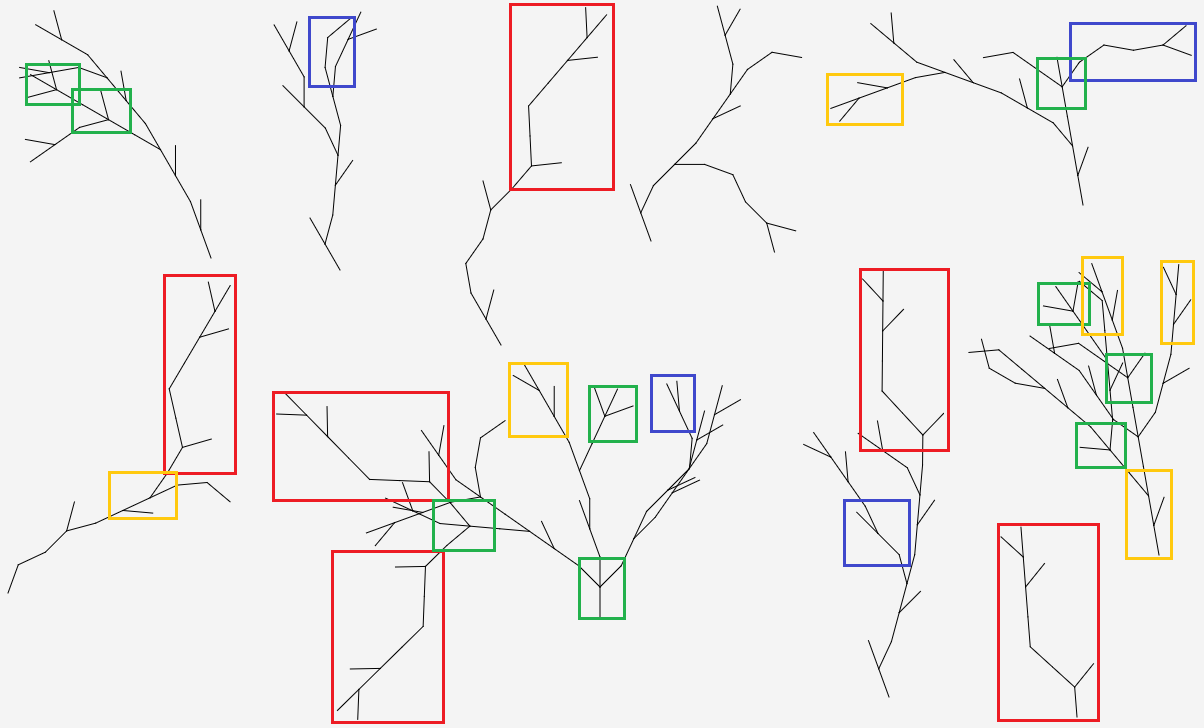
\includegraphics[width=14.5cm]{../images/synthesis_marks.png}
    \caption{Untersuchung der synthetisierten Verzweigungsstrukturen}
\end{figure}


\subsection*{Auswirkung der Gewichtungsparameter}
Der Parameter $w_l$ des vorgestellten Komprimierungsalgorithmus gewichtet eine Funktion,
welche die Kosten eines L-Systems ermittelt, sodass der Algorithmus L-Systeme mit unterschiedlich
großer Produktionsregelmenge anders behandelt.
Hierbei bewertet ein Wert von $0.0$ eine große Produktionsregelmenge höher.
Entspricht $w_l$ einem Wert von $1.0$, wird eine kleinere Produktionsregelmenge überbewertet.
Der Durchschnittswert $0.5$, der im Beispiel verwendet wird, sorgt für eine moderate Menge an
Produktionsregeln bei moderater Länge der einzelnen Regel.
Der im Generalisierungsalgorithmus vorgestellte Gewichtungsparameter $w_0$ legt fest, inwiefern
die Länge oder \textit{String Edit Distance} zweier Grammatiken von Bedeutung sind.
Bei einem Wert von $0.0$ überbewertet der Algorithmus die Metrik zur Berechnung der Anzahl Operationen,
um eine Grammatik in eine zweite zu überführen.
Der Wert $1.0$ entspricht einer Überbewertung der Längenmetrik.
Im Beispiel wird der Durchschnittswert $0.5$ verwendet.

$w_l$ und $w_0$ sind im Programm als \textit{Rula application ratio} und \textit{Merge application ratio}
bezeichnet und können vom Benutzer vor der Generierung festgelegt werden.

%Folgende Tabelle zeigt die Wahl der Gewichtungsparameter und gibt ein zugehöriges Beispiel an:
%\begin{figure}[H]
%    \centering
%    \begin{tabular}{|l|c|c|}\hline
%    \diagbox[width=10em]{$w_l$}{$w_0$} & Niedrig & Hoch \\ \hline
%    Niedrig & Beispiel 1 & Beispiel 2 \\ \hline
%    Hoch & Beispiel 3 & Beispiel 4 \\ \hline
%    \end{tabular}
%    \caption{Wahl der Gewichtungsparameter}
%\end{figure}
%
%\begin{figure}[H]
%    \centering
%    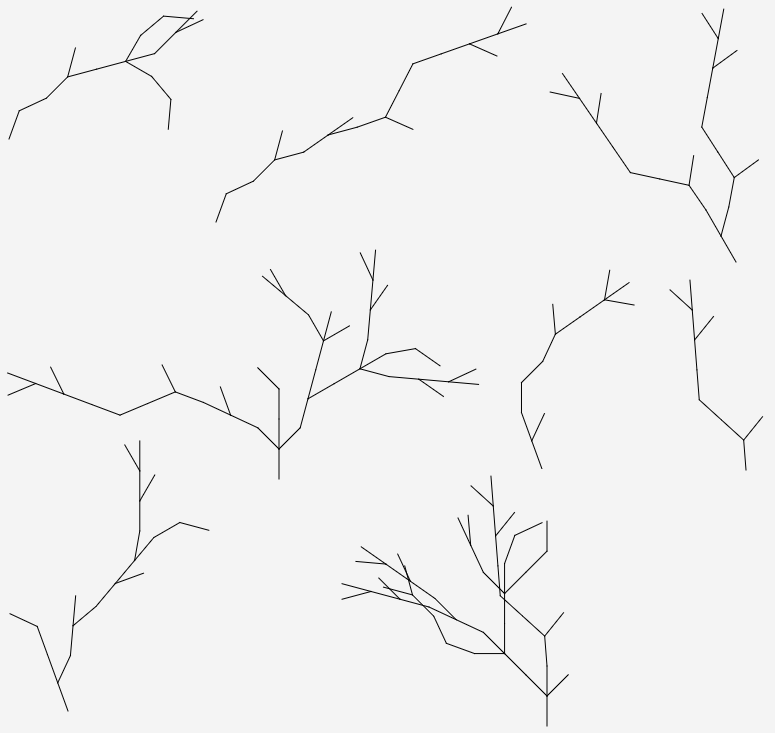
\includegraphics[width=9cm]{../images/low_low.png}
%    \caption{\underline{Beispiel 1}: $w_l=0.1$, $w_0=0.1$}
%\end{figure}
%\begin{figure}[H]
%    \centering
%    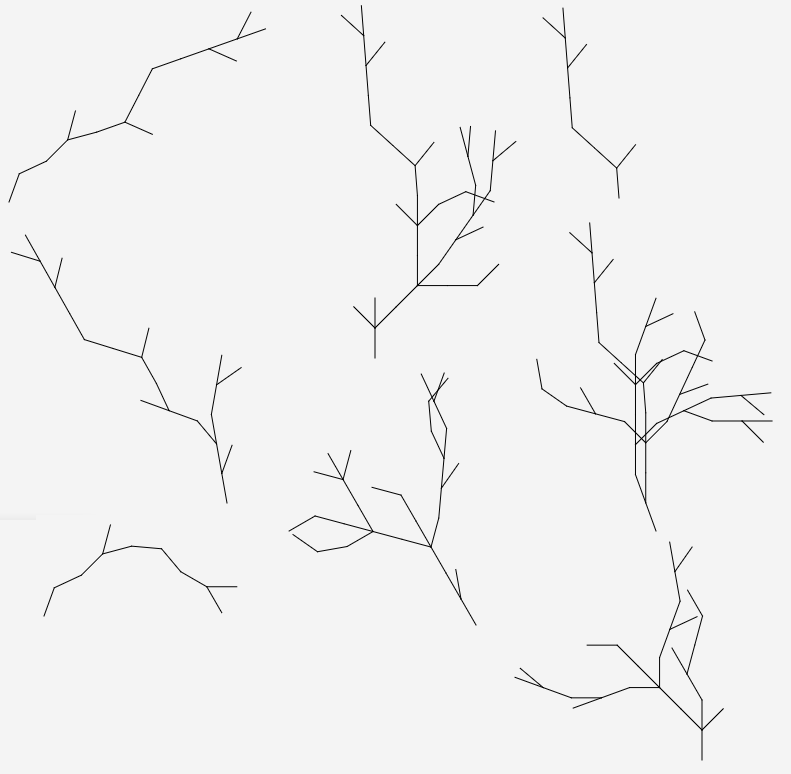
\includegraphics[width=9cm]{../images/low_high.png}
%    \caption{\underline{Beispiel 2}: $w_l=0.1$, $w_0=0.9$}
%\end{figure}
%\begin{figure}[H]
%    \centering
%    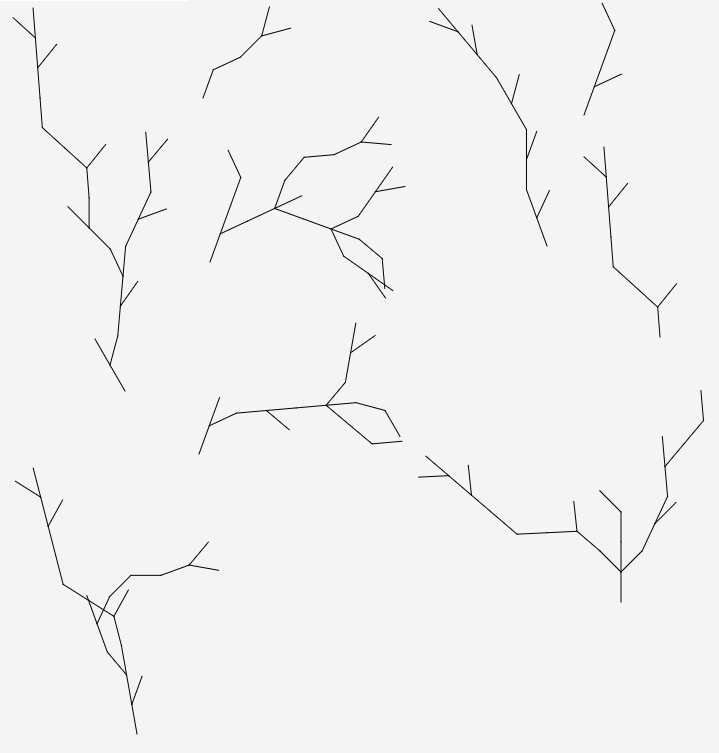
\includegraphics[width=9cm]{../images/high_low.png}
%    \caption{\underline{Beispiel 3}: $w_l=0.9$, $w_0=0.1$}
%\end{figure}
%\begin{figure}[H]
%    \centering
%    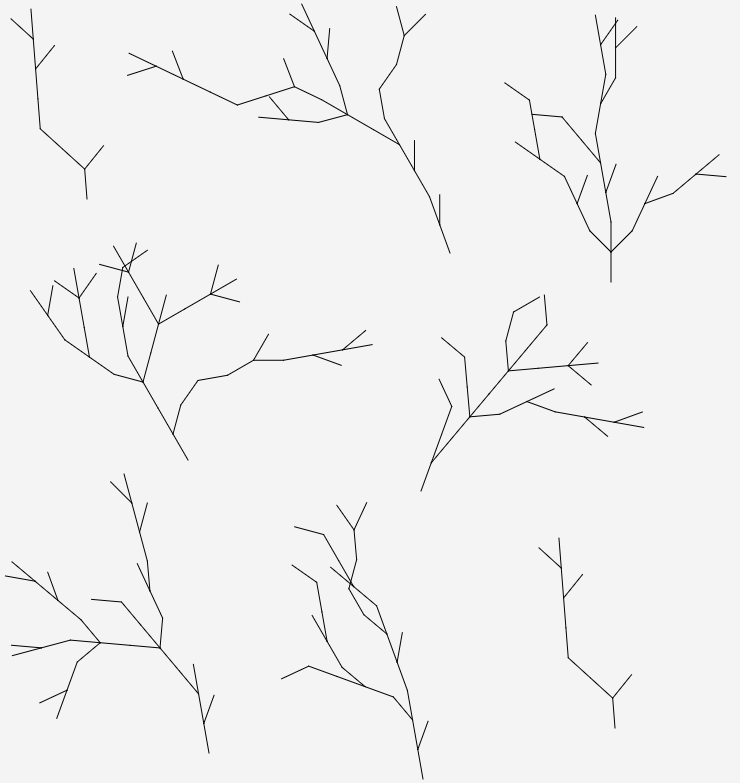
\includegraphics[width=9cm]{../images/high_high.png}
%    \caption{\underline{Beispiel 4}: $w_l=0.9$, $w_0=0.9$}
%\end{figure}
% @author Arian Helberg

\chapter{Fazit und Ausblick}
Diese Arbeit beschreibt die Konzeption und Implementierung eines prozeduralen Systems zur Erstellung
von Verzweigungsstrukturen, die einer Eingabestruktur ähneln.
Dabei werden Anforderungen untersucht, die zur Erstellung einer individuellen Software nötig sind.
Eine intuitiv nutzbare Anwendung zur benutzergesteuerten Strukturierung von eingelesenen Templates und
anschließender Generierung von Ähnlichkeitsstrukturen, ist im Rahmen dieser Arbeit entstanden.

\subsection*{Fazit}
Diese Arbeit zeigt, wie Ansätze der aktuellen Forschung genutzt werden können, um Verzweigungsstrukturen
zu erzeugen.
L-Systeme eignen sich gut, um Verzweigungsstrukturen mathematisch zu beschreiben und so in einem
Programm zu verwenden.
Sie können durch Ausführung und Interpretation durch einen Logo-Turtle-Algorithmus visualisiert
und mittels grafischer Bedienelemente sichtbar gemacht werden.
Die Steuerung von Gewichtungsparametern durch den Benutzer verhindert unnötige
\textit{Trial and Error}-Szenarien, da das Ergebnis des Prozesses gesteuert werden kann.
Die Erstellung und Integration eines neuronalen Netzes, das laut aktueller Forschung gute Ergebnisse beim Lernen von
Regeln aus einer Eingabestruktur liefert, kann in dieser Arbeiten aus Praktikabilitätsgründen nicht behandelt werden.\\
Die umgesetzte Softwaretechnik zur Erstellung des Softwareprojekts stellt sich bedingt als praktikabel
heraus.
Auf der einen Seite ist ein gewisses Maß an Expertise in der Java-Spezifikation JavaFX nötig, um
die Implementierung mit einem test-driven Ansatz zu beginnen.
Weiter ist die Erreichung einer ausreichenden Testabdeckung mit Modultests nur schwer
zu erreichen, da einige Module eine lauffähige JavaFX-Instanz benötigen.
Auf der anderen Seite hilft sie eine angemessene Testabdeckung und so hochwertigen Quellcode
zu erzeugen.
Darüber hinaus ist das Softwareprojekt durch den Ansatz gut strukturiert und verringert
den Aufbau technischer Schuld.

\subsection*{Ausblick}
Die Eingabestrukturen lassen sich ohne erneute Konzeptionierung in andere Strukturen, die ebenfalls
einer Baumtopologie entsprechen, überführen.
L-Systeme beschreiben Baumstrukturen grundlegend und können diese durch deren Auflösung visualisieren.
So können bspw. Websites, die durch das \textit{DOM} spezifiziert sind, auf diese Weise interpretiert
und erstellt werden.
Hierzu muss die Software um eine Bereitstellung des erzeugten, generalisierten L-Systems erweitert
werden.\\
Eine Weiterführung des Softwareprojekts kann durch den Einsatz neuronaler Netze zum Lernen
struktureller Regeln und Ableiten von Transformationsparametern erreicht werden.
Auf der einen Seite lässt sich die Erstellung von Ähnlichkeitsstrukturen durch neuronale Netze
automatisieren und vereinfachen, auf der anderen Seite entsteht dadurch ein initialer Mehraufwand
der Implementierung.\\
Weiter lassen sich die Konzepte zur Synthese zweidimensionaler Strukturen in zukünftigen Arbeiten
in den dreidimensionalen Raum überführen.
Zum Schluss ist das Erkennen von Überlappungen von Strukturen ein schwieriges Problem der
Computergrafik und kann durch zusätzliche Algorithmen umgesetzt werden.
% Add additional chapters here

%\bibliographystyle{plain}
\bibliographystyle{dinat}
\bibliography{literature}

% Appendix
\appendix
% !TEX root = ../thesis.tex
% appendix example chapter
% @author Thomas Lehmann
%
\chapter{Anhang}


\IGlossary

\Istatement

\end{document}
